% Dependencias ---------------------------------------------------------
\documentclass[12pt, letterpaper, oneside, openany, final]{book} 
\usepackage[spanish,es-tabla,es-nodecimaldot, es-nosectiondot, es-lcroman, es-noquoting]{babel}
\let\quoting\relax\let\endquoting\relax
\usepackage[T1]{fontenc}
\usepackage{newtxtext} % Time new roman
\usepackage{newtxmath}
\usepackage[utf8]{inputenc}
\usepackage[final]{microtype}
\usepackage{blindtext}

\usepackage{datetime}
	\newdateformat{monthyeardate}{%
		\monthname[\THEMONTH] de \THEYEAR}

\usepackage{datetime}
	\newdateformat{daymonthyeardate}{%
		\THEDAY de \monthname[\THEMONTH] de \THEYEAR}

\usepackage[right=3cm, left=4cm, top=3cm, bottom=3cm, nohead=true, foot=20pt,
includefoot, heightrounded]{geometry}

\usepackage{graphicx}
	\graphicspath{ {imagenes/} }

\usepackage[export]{adjustbox}
	\setcounter{section}{0}

\usepackage[chapter]{minted}
	\renewcommand\listingscaption{Codigo}
	
\usepackage{anyfontsize}
\usepackage[svgnames]{xcolor}
	\definecolor{resaltado}{RGB}{204,255,0}

\usepackage[numbib]{tocbibind}
	% notlof = no lista de figuras en el indice
	% numbib = Number the Bibliography heading
	% notlot = Disables the inclusion of the List of Tables

\usepackage{chngcntr}
	
\usepackage[font=small,labelfont=bf,hypcap=true]{caption}
\usepackage{subcaption}

\usepackage{array}
\usepackage{booktabs}
	\setlength\heavyrulewidth{0.9pt}

\usepackage{threeparttable}

\usepackage{scrextend}
\usepackage{amsmath}
\usepackage{nccmath}

\usepackage[style=american,thresholdtype=words, parthreshold=true]{csquotes}
	\SetBlockThreshold{40}

\usepackage[vskip=10pt, leftmargin=\parindent, rightmargin=\parindent, 	indentfirst=false]{quoting}
	\AtBeginEnvironment{quoting}{\singlespacing}
	\SetBlockEnvironment{quoting}

\usepackage[style=apa, backend=biber]{biblatex}
	\addbibresource{referencias.bib}
	\setlength\bibitemsep{4\itemsep}
	\DefineBibliographyStrings{spanish}{andothers={et al\adddot}}
	%\DeclareLanguageMapping{spanish}{american-apa}
	\DeclareLanguageMapping{spanish}{spanish-apa}

\usepackage{pdfpages}
\usepackage{setspace} 	% Interlineado
\usepackage{longtable, tabu}
\usepackage{csvsimple}
\usepackage{lscape}
\usepackage{parskip}

\usepackage[bottom]{footmisc}
\usepackage[all]{nowidow}		% para evitar lineas huerfanas y viudas
	%\widowpenalty = 10000
	%\clubpenalty = 10000
	%\postdisplaypenalty = 10000
\usepackage{datatool} 	% para el sortedlist en el glosario
\usepackage{etoolbox}
\usepackage{enumitem}
	\setlist{nolistsep}
\usepackage{titlesec}
\usepackage{titletoc}% http://ctan.org/pkg/titletoc
\usepackage{fancyhdr}
\usepackage{xpatch}
\usepackage{afterpage}
\usepackage{flafter}
\usepackage{dblfloatfix}

\usepackage{draftwatermark}
%\usepackage[nostamp]{draftwatermark}
	\SetWatermarkText{NO FINAL}
	\SetWatermarkScale{0.8}
	\SetWatermarkLightness{0.96}

\usepackage[colorlinks = true,
			linkcolor = black,
			urlcolor = blue,
			citecolor = black,
			hyperfootnotes = true,
			pdfstartview=XYZ]{hyperref}
			
			% pdfstartview=XYZ para ajustar la pagina
			% pdfpagelayout=SinglePage para landscape vertical

\usepackage[nameinlink, noabbrev, spanish, capitalize]{cleveref}

% Para la separacion de ecuaciones
\makeatletter
\g@addto@macro\normalsize{\setlength\abovedisplayshortskip{0pt}}
\g@addto@macro\normalsize{\setlength\belowdisplayshortskip{0pt}}
\g@addto@macro\normalsize{\setlength\abovedisplayskip{17pt}}
\g@addto@macro\normalsize{\setlength\belowdisplayskip{10pt}}
\makeatother

% Formato tesis unet

\addto\captionsspanish{\renewcommand{\contentsname}%
	{ÍNDICE}%
}

\addto\captionsspanish{\renewcommand{\listtablename}%
	{ÍNDICE DE TABLAS}%
}

\addto\captionsspanish{\renewcommand{\listfigurename}%
	{ÍNDICE DE FIGURAS}%
}

\addto\captionsspanish{\renewcommand{\listoflistingscaption}
	{ÍNDICE DE CODIGOS}%
}


\crefname{equation}{}{}
\crefname{listing}{Código}{Códigos}
\crefname{table}{\spanishtablename}{\spanishtablename}
\newcommand{\addperiod}[1]{#1.$\enspace$}

% --------------------------------------------
% FORMATO UNET -------------------------------

\newcommand{\UnetFormat}{
	
	\counterwithout{figure}{chapter}
	\counterwithout{table}{chapter}
	\counterwithout{equation}{chapter}
	\counterwithout{listing}{chapter}
	\setcounter{tocdepth}{1}
	\setcounter{secnumdepth}{0}
	
	\renewcommand{\thechapter}{\Roman{chapter}}
	\titleformat{\section}[block]{\centering\normalsize\bfseries}{\thesection}{1em}{}
	\titleformat{\subsection}[block]{\centering\normalsize\bfseries\itshape}{\thesubsection}{1em}{}
	\titleformat{\subsubsection}[block]{\normalsize\bfseries\itshape}{\thesubsubsection}{1em}{}
	\titleformat{\paragraph}[runin]{\normalsize\bfseries\itshape }{\theparagraph}{1em}{\addperiod}
	
	\titlespacing\section{0pt}{20pt plus 4pt minus 4pt}{20pt plus 4pt minus 4pt}
	\titlespacing\subsection{0pt}{10pt plus 4pt minus 4pt}{10pt plus 4pt minus 4pt}
	\titlespacing\subsubsection{0pt}{10pt plus 4pt minus 4pt}{10pt plus 4pt minus 4pt}
	\titlespacing{\paragraph}{1.5cm}{10pt plus 0pt minus 4pt}{0pt plus 0pt minus 0pt}
	
	% setup de caption y ambiente de tablas
	\captionsetup[table]{textfont=bf, format=plain, justification=justified, singlelinecheck=false, labelsep=spaced, belowskip=0pt, aboveskip=1pt}
		
	% setup de caption y ambiente de figuras
	\captionsetup[figure]{labelformat=simple,labelsep=period, labelfont=bf, textfont=footnotesize, justification=justified, singlelinecheck=false, belowskip=-10pt}
	
	\captionsetup[subfigure]{labelsep=period, labelfont=bf, textfont=normal, justification=centering, singlelinecheck=false, belowskip=0pt}
	
	\setlength{\textfloatsep}{15pt plus 1.0pt minus 2.0pt}
	\setlength{\floatsep}{15pt plus 1.0pt minus 2.0pt}
	\setlength{\intextsep}{15pt plus 1.0pt minus 2.0pt} 
	
	\captionsetup[listing]{format=plain, justification=justified, singlelinecheck=false, labelsep=period, belowskip=10pt, aboveskip=10pt}
	

	% Configuracion del TOC	
	\titlecontents{section}% <section-type>
		[1.5cm]% <left>
		{\addvspace{-2pt}}% <above-code>
		{\makebox[0.78cm][l]{\thecontentslabel}\hspace{1.7em}}% <numbered-entry-format>
		{}% <numberless-entry-format>
		{\titlerule*[8pt]{.}\contentspage}[\addvspace{-2pt}]

	\titlecontents{subsection}% <section-type>
		[3cm]% <left>
		{\addvspace{-2pt}}% <above-code>
		{\makebox[0.63cm][l]{\thecontentslabel}\hspace{2.1em}}% <numbered-entry-format>
		{}% <numberless-entry-format>
		{\titlerule*[8pt]{.}\contentspage}[\addvspace{-2pt}]

	\titlecontents{subsubsection}% <section-type>
		[4.5cm]% <left>
		{\addvspace{-2pt}}% <above-code>
		{\makebox[20pt][l]{\thecontentslabel}\hspace{3.1em}}% <numbered-entry-format>
		{}% <numberless-entry-format>
		{\titlerule*[8pt]{.}\contentspage}[\addvspace{-2pt}]

	\titlecontents{paragraph}% <section-type>
		[6.52cm]% <left>
		{\addvspace{0pt}}% <above-code>
		{\makebox[20pt][l]{\thecontentslabel}\qquad\qquad}% <numbered-entry-format>
		{}% <numberless-entry-format>
		{\titlerule*[8pt]{.}\contentspage}[\addvspace{0pt}]

}

% FORMATO UNET FIN ---------------------------
% --------------------------------------------

% --------------------------------------------
% FORMATO NUMERADO ---------------------------

\newcommand{\NumeradoFormat}{
	
	\setcounter{tocdepth}{4}
	\setcounter{secnumdepth}{4}
	\renewcommand{\thechapter}{\Roman{chapter}}
	
	\renewcommand{\thesection}{\arabic{chapter}.\arabic{section}}
	\renewcommand{\thesubsection}{\arabic{chapter}.\arabic{section}.\arabic{subsection}}
	\renewcommand{\thesubsubsection}{\arabic{chapter}.\arabic{section}.\arabic{subsection}.\arabic{subsubsection}}
	\renewcommand{\theparagraph}{\arabic{chapter}.\arabic{section}.\arabic{subsection}.\arabic{subsubsection}.\arabic{paragraph}}
	\renewcommand{\thefigure}{\arabic{chapter}.\arabic{figure}}
	\renewcommand{\thetable}{\arabic{chapter}.\arabic{table}}
	\renewcommand{\theequation}{\arabic{chapter}.\arabic{equation}}
	\renewcommand{\thelisting}{\arabic{chapter}.\arabic{listing}}
	
	\titleformat{\section}[block]{\normalsize\bfseries}{\thesection}{1em}{}
	\titleformat{\subsection}[block]{\normalsize\bfseries}{\thesubsection}{1em}{}
	\titleformat{\subsubsection}[block]{\normalsize\bfseries\itshape}{\thesubsubsection}{1em}{}
	\titleformat{\paragraph}[runin]{\normalsize\bfseries\itshape }{\theparagraph}{1em}{\addperiod}
	
	\titlespacing\section{0pt}{20pt plus 4pt minus 4pt}{20pt plus 4pt minus 4pt}
	\titlespacing\subsection{1.5cm}{10pt plus 4pt minus 4pt}{10pt plus 4pt minus 4pt}
	\titlespacing\subsubsection{1.5cm}{10pt plus 4pt minus 4pt}{10pt plus 4pt minus 4pt}
	\titlespacing{\paragraph}{1.5cm}{10pt plus 0pt minus 4pt}{0pt plus 4pt minus 4pt}
	
	% setup de caption y ambiente de tablas
	\captionsetup[table]{textfont=bf, format=plain, justification=justified, singlelinecheck=false, labelsep=spaced, belowskip=0pt, aboveskip=1pt}
	
	% setup de caption y ambiente de figuras
	\captionsetup[figure]{labelformat=simple,labelsep=period, labelfont=bf, textfont=footnotesize, justification=justified, singlelinecheck=false, belowskip=-10pt}
	
	\captionsetup[subfigure]{labelsep=period, labelfont=bf, textfont=normal, justification=centering, singlelinecheck=false, belowskip=0pt}
	
	\setlength{\textfloatsep}{15pt plus 1.0pt minus 2.0pt}
	\setlength{\floatsep}{15pt plus 1.0pt minus 2.0pt}
	\setlength{\intextsep}{15pt plus 1.0pt minus 2.0pt}
	
	\captionsetup[listing]{format=plain, justification=centering, singlelinecheck=false, labelsep=period, belowskip=10pt, aboveskip=10pt}
	
	% Configuracion del TOC
	\newlength\sectionlenght
	\setlength{\sectionlenght}{-0.5cm - \widthof{\thesection}}

	\newlength\subsectionlenght
	\setlength{\subsectionlenght}{-0.5cm - \widthof{\thesubsection}}

	\newlength\subsubsectionlenght
	\setlength{\subsubsectionlenght}{-0.5cm - \widthof{\thesubsubsection}}

	\newlength\paragraphlenght
	\setlength{\paragraphlenght}{-0.5cm - \widthof{\theparagraph}}

	\titlecontents{section}% <section-type>
		[0.5cm + \widthof{\thesection}]% <left>
		{\addvspace{-2pt}}% <above-code>
		{\hspace{\sectionlenght}\makebox[\widthof{\thecontentslabel}][l]{\thecontentslabel}\hspace{0.5cm}}% <numbered-entry-format>
		{}% <numberless-entry-format>
		{\titlerule*[8pt]{.}\contentspage}[\addvspace{-2pt}]
	
	\titlecontents{subsection}% <section-type>
		[0.5cm + \widthof{\thesection} + 0.5cm + \widthof{\thesubsection}]% <left>
		{\addvspace{-2pt}}% <above-code>
		{\hspace{\subsectionlenght}\makebox[\widthof{\thecontentslabel}][l]{\thecontentslabel}\hspace{0.5cm}}% <numbered-entry-format>
		{}% <numberless-entry-format>
		{\titlerule*[8pt]{.}\contentspage}[\addvspace{-2pt}]
		
	\titlecontents{subsubsection}% <section-type>
		[1cm + \widthof{\thesection} + \widthof{\thesubsection} + 0.5cm + \widthof{\thesubsubsection}]% <left>
		{\addvspace{-2pt}}% <above-code>
		{\hspace{\subsubsectionlenght}\makebox[\widthof{\thecontentslabel}][l]{\thecontentslabel}\hspace{0.5cm}}% <numbered-entry-format>
		{}% <numberless-entry-format>
		{\titlerule*[8pt]{.}\contentspage}[\addvspace{-2pt}]
		
	\titlecontents{paragraph}% <section-type>
		[1.5cm + \widthof{\thesection} + \widthof{\thesubsection} + \widthof{\thesubsubsection} + 0.5cm + \widthof{\theparagraph}]% <left>
		{\addvspace{0pt}}% <above-code>
		{\hspace{\paragraphlenght}\makebox[\widthof{\thecontentslabel}][l]{\thecontentslabel}\hspace{0.5cm}}% <numbered-entry-format>
		{}% <numberless-entry-format>
		{\titlerule*[8pt]{.}\contentspage}[\addvspace{0pt}]
}

% FORMATO NUMERADO FIN -----------------------
% --------------------------------------------


% incio de macro para cambiar chapter al centro
\newcommand{\Centerformat}{
	\titleformat{\chapter}[display]
	{\large\bfseries\centering}{\MakeUppercase{\chaptertitlename\ \thechapter}}{0pt}{\large\MakeUppercase}
	\titlespacing{\chapter}
	{0pt}{-5pt}{20pt}
	
	\titlecontents{chapter}% <section-type>
		[3.22cm]% <left>
		{\addvspace{7pt}}% <above-code>
		{\hspace{-3.22cm}\MakeUppercase{\bfseries\chaptername}\hspace{0.1em}
		\makebox[10pt][l]{\bfseries\thecontentslabel}\bfseries\quad\uppercase}% <numbered-entry-format>
		{\hspace{-3.22cm}\bfseries\uppercase}% <numberless-entry-format>
		{\hfill\contentspage}[\addvspace{7pt}]
}

% ---------------------------------------------------------------------

% incio de macro para cambiar chapter a la izquierda
\newcommand{\CenterformatBack}{
	\titleformat{\chapter}[display]
	{\large\bfseries\centering}{\MakeUppercase{\chaptertitlename\ \thechapter}}{0pt}{\large}
	\titlespacing{\chapter}
	{0pt}{-20pt}{30pt}
	
	\titlecontents{chapter}% <section-type>
		[0pt]% <left>
		{\addvspace{0pt}}% <above-code>
		{}% <numbered-entry-format>
		{\bfseries\normalsize\uppercase}% <numberless-entry-format>
		{\titlerule*[8pt]{.}\contentspage}[\addvspace{0pt}]
}

% incio de macro para cambiar chapter frente
\newcommand{\CenterformatFront}{
	\titleformat{\chapter}[display]
	{\large\bfseries\centering}{\MakeUppercase{\chaptertitlename\ \thechapter}}{0pt}{\large}
	\titlespacing{\chapter}
	{0pt}{-10pt}{0pt}
	
	\titlecontents{chapter}% <section-type>
		[0pt]% <left>
		{\addvspace{0pt}}% <above-code>
		{}% <numbered-entry-format>
		{\bfseries\normalsize\uppercase}% <numberless-entry-format>
		{\titlerule*[8pt]{.}\contentspage}[\addvspace{0pt}]
}

% ---------------------------------------------------------------------

%\let\svsubsubsection\subsubsection %separacion del bloque de texto por seccion
%\def\subsubsection{\leftskip 1.25cm\svsubsubsection} 

%\BeforeBeginEnvironment{equation}{\vspace{7pt}}
%\AfterEndEnvironment{equation}{\leavevmode}

\BeforeBeginEnvironment{align}{\vspace{-10pt}}
\AfterEndEnvironment{align}{\vspace{-30pt}\leavevmode}

\BeforeBeginEnvironment{minted}{\vspace*{-7pt}}
\AfterEndEnvironment{minted}{\vspace*{-30pt}\leavevmode}

% ---------------------------------------------------------------------

\setlist[itemize]{leftmargin=1.25cm}

%Inicio del macro para el sortdlist ( ordenar un itemize ) ------------
\newcommand{\sortitem}[2][\relax]{%
	\DTLnewrow{list}% Create a new entry
	\ifx#1\relax
	\DTLnewdbentry{list}{sortlabel}{#2}% Add entry sortlabel (no optional argument)
	\else
	\DTLnewdbentry{list}{sortlabel}{#1}% Add entry sortlabel (optional argument)
	\fi%
	\DTLnewdbentry{list}{description}{#2}% Add entry description
}
\newenvironment{sortedlist}{%
	\DTLifdbexists{list}{\DTLcleardb{list}}{\DTLnewdb{list}}% Create new/discard old list
}{%
	\DTLsort{sortlabel}{list}% Sort list
	\begin{itemize}[label={}, leftmargin=0pt, labelwidth=0pt, labelsep=0pt]%
		\DTLforeach*{list}{\theDesc=description}{%
			\item \theDesc}% Print each item
	\end{itemize}%
}
% ---------------------------------------------------------------------

% para modificar el ambiente " qoute "
%\AtBeginEnvironment{quote}{\addtolength\leftmargini{1.25cm}}

% Para modificar el Y en las referencias y bibliografia
\DeclareDelimFormat*{finalnamedelim}
{\ifnum\value{liststop}>2 \finalandcomma\fi\addspace y \space}

% the bibliography also needs another conditional, so we can't wrap
% everything up with just the two lines above
\DeclareDelimFormat[bib,biblist]{finalnamedelim}{%
	\ifthenelse{\value{listcount}>\maxprtauth}
	{}
	{\ifthenelse{\value{liststop}>2}
		{\finalandcomma\addspace y \space}
		{\addspace y \space}}}

% this is a special delimiter to solve the bugs reported in
% https://tex.stackexchange.com/q/417648/35864
\DeclareDelimFormat*{finalnamedelim:apa:family-given}{%
	\ifthenelse{\value{listcount}>\maxprtauth}
	{}
	{\finalandcomma\addspace y\space}}

\DeclareCaptionLabelSeparator*{spaced}{.\\}
\DeclareCaptionLabelFormat{numero}{\textbf{#1 #2}}

% Con encabezado y pie de pagina
\newcommand{\Addheadfoot}{
\newgeometry{right=3cm, left=4cm, top=3cm, bottom=3cm, includeheadfoot, headheight=15pt, heightrounded}
	\newcommand{\MainStyle}{
		\fancypagestyle{Main}{
			\fancyhf{}% clear all fields
			\renewcommand{\headrulewidth}{0.4pt}%
			\renewcommand{\footrulewidth}{0.4pt}
			\rhead{\rightmark}
			\lhead{\leftmark}
			\rfoot{Autor: Kleiver Carrasco}%
			\cfoot{\thepage}
		}
	
		\fancypagestyle{plain}{% for the chapter start pages
			\fancyhf{}% clear all fields
			\renewcommand{\headrulewidth}{0pt}%
			\renewcommand{\footrulewidth}{0.4pt}
			\rfoot{Autor: Kleiver Carrasco}%
			\cfoot{\thepage}
		}
	
		\pagestyle{Main}
	}
	
	\newcommand{\FrontBackStyle}{
		\fancypagestyle{plain}{% for the chapter start pages
			\fancyhf{}% clear all fields
			\renewcommand{\headrulewidth}{0pt}%
			\renewcommand{\footrulewidth}{0pt}
			\fancyfoot[C]{\thepage}%
		}
	
		\pagestyle{plain}
	}
}

% sin encabezado y sin pie de pagina
\newcommand{\noAddheadfoot}{
	
	\newcommand{\FrontBackStyle}{
		\fancypagestyle{plain}{% for the chapter start pages
			\fancyhf{}% clear all fields
			\renewcommand{\headrulewidth}{0pt}%
			\renewcommand{\footrulewidth}{0pt}
			\fancyfoot[C]{\thepage}%
		}
		
		\pagestyle{plain}}
	
	\newcommand{\MainStyle}{
		\fancypagestyle{Main}{% for the chapter start pages
			\fancyhf{}% clear all fields
			\renewcommand{\headrulewidth}{0pt}%
			\renewcommand{\footrulewidth}{0pt}
			\fancyfoot[C]{\thepage}%
		}
		
		\pagestyle{Main}}
}

% Solo encabezado
\newcommand{\AddheadOnly}{
	\newgeometry{right=3cm, left=4cm, top=3cm, bottom=3cm, includeheadfoot, heightrounded}
	\newcommand{\MainStyle}{
		\fancypagestyle{Main}{
			\fancyhf{}% clear all fields
			\renewcommand{\headrulewidth}{0.4pt}%
			\renewcommand{\footrulewidth}{0pt}
			\rhead{}
			\lhead{\leftmark}
			\cfoot{\thepage}
		}
		
		\fancypagestyle{plain}{% for the chapter start pages
			\fancyhf{}% clear all fields
			\renewcommand{\headrulewidth}{0pt}%
			\renewcommand{\footrulewidth}{0pt}
			\cfoot{\thepage}
		}
		
		\pagestyle{Main}
	}
	
	\newcommand{\FrontBackStyle}{
		\fancypagestyle{plain}{% for the chapter start pages
			\fancyhf{}% clear all fields
			\renewcommand{\headrulewidth}{0pt}%
			\renewcommand{\footrulewidth}{0pt}
			\fancyfoot[C]{\thepage}%
		}
		
		\pagestyle{plain}
	}
}

\addtocontents{toc}{~\hfill\par}
\addtocontents{toc}{~\hfill Pág.\par}
\addtocontents{toc}{~\hfill\par}
%\addtocontents{toc}{\protect\afterpage{~\hfill Pág.\par\medskip}}

\addtocontents{lof}{~\hfill\par}
\addtocontents{lof}{FIGURA~\hfill Pág.\par}
\addtocontents{lof}{~\hfill\par}
%\addtocontents{lof}{\protect\afterpage{~\hfill Pag.\par\medskip}}

\addtocontents{lot}{~\hfill\par}
\addtocontents{lot}{TABLA~\hfill Pág.\par}
\addtocontents{lot}{~\hfill\par}
%\addtocontents{lot}{\protect\afterpage{~\hfill Pag.\par\medskip}}

\addtocontents{lol}{~\hfill\par}
\addtocontents{lol}{CÓDIGO~\hfill Pág.\par}
\addtocontents{lol}{~\hfill\par}
%\addtocontents{lol}{\protect\afterpage{~\hfill Pag.\par\medskip}}

\renewcommand{\listoflistings}{%
	\cleardoublepage
	\phantomsection
	\addcontentsline{toc}{chapter}{\protect\listoflistingscaption}%
	\listof{listing}{\listoflistingscaption}%
	\newpage
	
}

\newcommand*{\noaddvspace}{\renewcommand*{\addvspace}[1]{}}
\addtocontents{lof}{\protect\noaddvspace}
\addtocontents{lot}{\protect\noaddvspace}
\let\Chapter\chapter
\def\chapter{\addtocontents{lol}{\protect\addvspace{0pt}}\Chapter}


% Para arreglar el spacing en el ambiente quoting
\makeatletter
\renewcommand*\singlespacing{%
	\par    % ensure vertical mode
	\null   % add fake line with previous leading still in force
	\setstretch {\setspace@singlespace}% change leading
	\nobreak
	\vskip -\baselineskip   % compensate for the fake line we added, but with 
	% the new leading
	\vskip \z@skip  % tell "\addvspace" and "\addpenalty" _not_ to remove the 
	% above correction
}
\makeatother

\addto\captionsspanish{%
  \renewcommand\appendixname{Anexo}
  \renewcommand\appendixpagename{Anexos}
}

%\Addheadfoot
%\AddheadOnly
\noAddheadfoot

\begin{document}
%Portada ---------------------------------------------------------------
\begin{titlepage}
\pagenumbering{roman}
\begin{center}
	% Logo de la unet --------------------------------------------
	
\includegraphics[width=2cm]{unet.jpg}
	
	Universidad Nacional Experimental del Táchira 
	
	Vicerrectorado Académico
	
	Decanato de Docencia
	
	Departamento de Ingeniería Electrónica
	
	Trabajo de Aplicación Profesional
	
	Proyecto Especial de Grado
\end{center}

% Titulo central ---------------------------------------------
\centering
	\vspace{2.5cm}
	\vfill
	{\Large \textbf{Laboratorio virtual de sistemas de control clásicos y difusos utilizando software libre}\par}

% Autores ----------------------------------------------------
\vfill
\begin{flushright}
	\begin{spacing}{1.5}
		\textbf{Autor:} Kleiver J. Carrasco M.
		
		C.I: V-24.743.884
		
		\href{kleiver.carrasco@unet.edu.ve}{kleiver.carrasco@unet.edu.ve}
		
		\textbf{Tutor:} Juan R. Vizcaya R.
		
		\href{jvizcaya@unet.edu.ve}{jvizcaya@unet.edu.ve}
	\end{spacing}	
\end{flushright}

%Fecha ------------------------------------------------------
\vfill
	San Cristóbal, \monthyeardate\today
\leavevmode
\end{titlepage}
\begin{titlepage}
\parskip=7.25pt plus 2pt
\setcounter{page}{2}
\begin{flushright}
	San Cristóbal, \today
\end{flushright}

\vspace{1cm}
\vfill

\begin{flushleft}
		\singlespacing
		\setlength{\parskip}{0pt}
		
		\textbf{Señores:}
		
		Miembros de la Comisión del Trabajo de Aplicación Profesional
		
		Departamento de Ingeniería Electrónica
		
\end{flushleft}

\vfill
\begin{spacing}{1.5}
	Yo, Kleiver Jesús Carrasco Márquez, titular de la cédula de identidad No. \mbox{V-24.743.884}, inscrito en el periodo académico 2019-1, estudiante del décimo semestre de la carrera de Ingeniería Electrónica, por medio de la presente someto a consideración de la Comisión de Trabajo de Aplicación Profesional de este departamento, la propuesta de Proyecto Especial de Grado titulada \enquote{\textbf{Laboratorio virtual de sistemas de control clásicos y difusos utilizando software libre}}, la cual se desarrollará bajo la tutoría del profesor Juan Rafael Vizcaya Rojas.
	
	Se anexan los recaudos exigidos, de acuerdo a lo dispuesto en la normativa para el Trabajo de Aplicación Profesional de la Universidad Nacional Experimental del Táchira. La fecha estimada de culminación del proyecto es el 6 de noviembre de 2019.
	
	Sin otro particular a que hacer referencia y en espera de su respuesta,
	
	\setlength{\parskip}{20pt} 
	
	\noindent Atentamente,
\end{spacing}

\vfill

\begin{center}
	
	\rule{6cm}{1pt}
	
	\vspace{0.2cm}
	
	\parskip=0pt plus 2pt
    
    \begin{spacing}{1}    
        Kleiver Jesús Carrasco Márquez
    
        C.I. V-24.743.884
    \end{spacing}
\end{center}

\vspace{0.5cm}

\end{titlepage}
\begin{titlepage}
\setcounter{page}{3}
\setlength{\parindent}{1.5cm}					% Sangría
\setlength{\parskip}{0pt}						% Espaciado

\begin{flushright}
	San Cristóbal, \today
\end{flushright}

\vspace{1cm}
\vfill

\begin{flushleft}
		\singlespacing
		
		\setlength{\parskip}{0pt}
		
		\textbf{Señores:}
		
		Miembros de la Comisión del Trabajo de Aplicación Profesional
		
		Departamento de Ingeniería Electrónica
		
\end{flushleft}

\vfill
\begin{spacing}{1.5}
	Yo, Juan Rafael Vizcaya Rojas, titular de la cédula de identidad No. \mbox{V-7.348.191}, de profesión ingeniero en electrónica, adscrito al departamento de Ingeniería Electrónica de la Universidad Nacional Experimental del Táchira en la categoría de Asociado y con dedicación exclusiva, por medio de la presente expreso mi conformidad y acepto la tutoría de la propuesta de Proyecto Especial de Grado titulada \enquote{\textbf{Laboratorio virtual de sistemas de control clásicos y difusos utilizando software libre}}, presentada por el bachiller Kleiver Jesús Carrasco Márquez, titular de la cédula de identidad No. \mbox{V-24.743.884}, para optar al título de Ingeniero en Electrónica en la Universidad Nacional Experimental del Táchira.
	
	Sin otro particular a que hacer referencia, me suscribo de usted,
	
	\setlength{\parskip}{20pt} 
	
	\noindent Atentamente,
\end{spacing}

\vfill

\begin{center}
	
	\rule{6cm}{1pt}
	
	\vspace{0.2cm}
	
	Juan Rafael Vizcaya Rojas
	
	\setlength{\parskip}{0pt}
	
	C.I. V-7.348.191
\end{center}

%Fecha ------------------------------------------------------
\vspace{0.5cm}
\end{titlepage}
\begin{titlepage}
\parskip=7.25pt plus 2pt
\setcounter{page}{4}
\begin{center}
	\begin{spacing}{1}
	% Logo de la unet --------------------------------------------
	
\includegraphics[width=2cm]{unet.jpg}
	
	Universidad Nacional Experimental del Táchira 
	
	Vicerrectorado Académico
	
	Decanato de Docencia
	
	Departamento de Ingeniería Electrónica
	
	Trabajo de Aplicación Profesional
	
	Proyecto Especial de Grado
	\end{spacing}
\end{center}

\vspace{0.5cm}

\begin{center}
		
		\textbf{Aprobación del Tutor para presentación de la Propuesta del Proyecto Especial de Grado}
		
\end{center}

\vspace{0.5cm}

\begin{spacing}{1.5}
	Yo, Juan Rafael Vizcaya Rojas, en mi carácter de Tutor del Proyecto Especial de Grado titulado \enquote{\textbf{Laboratorio virtual de sistemas de control clásicos y difusos utilizando software libre}}, presentado por el bachiller Kleiver Jesús Carrasco Márquez titular de la cédula de identidad No. \mbox{V-24.743.884} por medio de la presente autorizo la presentación de la Propuesta del Proyecto Especial de Grado, ante la Comisión del Trabajo de Aplicación Profesional del Departamento de Ingeniería Electrónica, en virtud de considerar que reúne los requisitos establecidos en el artículo 16 de las Normas para el Trabajo de Aplicación Profesional de la UNET.
\end{spacing}

\vfill

\begin{center}
	
	\rule{6cm}{1pt}
	
	\vspace{0.2cm}
	
	\parskip=0pt plus 2pt
    
    \begin{spacing}{1}
        Tutor
    
        Juan Rafael Vizcaya Rojas
    
        C.I. V-7.348.191
    \end{spacing}
\end{center}

\vspace{0.5cm}

\end{titlepage}
% Habilitar un solo Formato, ambos estan definidos en MacrosTesis.tex

\NumeradoFormat 	% Formato de titulos numerado con capitulos en romano
%\UnetFormat			% Formato de titulo basado en instructivo TAP

\frontmatter
\FrontBackStyle
\CenterformatFront
%\renewcommand{\chaptername}{Etapa}				% para cambiar de nombre
\spacing{1.6}									% interlineado del documento
\clearpage
\setcounter{page}{5}
\tableofcontents								% indice
%\newpage 										% habilitar para article
	\listoffigures								% Indice de tablas
	\listoftables

\renewcommand{\thefootnote}{(\arabic{footnote})}
\renewcommand{\labelitemi}{$\bullet$}
\setlength{\parindent}{1.5cm}					% Sangria
% \setlength{\parskip}{0pt}						% Espaciado
\parskip=0pt
\quotingsetup{leftmargin=\parindent, rightmargin=\parindent}


% Habilitar un solo Formato, ambos están definidos en configurationFile.tex

%\NumeradoFormat 	% Formato de títulos numerado con capítulos en romano
\UnetFormat			% Formato de titulo basado en instructivo TAP de la UNET
% ------------------------------------------------------------------------

%\frontmatter
\setcounter{secnumdepth}{-1}
\pagenumbering{roman}

\FrontBackStyle
\CenterformatFront

\setcounter{page}{5}					% Numero basado en paginas previas
\begin{center}
	\begin{spacing}{1}
		UNIVERSIDAD NACIONAL EXPERIMENTAL DEL TÁCHIRA
		
		VICERRECTORADO ACADÉMICO
		
		DECANATO DE DOCENCIA
		
		CARRERA DE INGENIERÍA ELECTRÓNICA
	
		\vspace{30pt}

		{\large \textbf{Laboratorio virtual de sistemas de control clásicos y difusos utilizando software libre}\par}
	
	\end{spacing}
\end{center}

\vspace{20pt}

\begin{flushright}
	\begin{spacing}{1}
		\parskip=0pt plus 1pt

		Autor: Kleiver J. Carrasco M.

		Tutor: MSc. Juan R. Vizcaya R.

		Fecha: Enero, 2020
		
	\end{spacing}	
\end{flushright}

\vspace{10pt}

\begin{abstract}
	\blindtext
	\blindtext
\end{abstract}

\keywords{Texto, sistemas de control, logica difusa}


\clearpage
\spacing{1.5} 							% interlineado de los indices
\tableofcontents						% indice
	\listoffigures						% Indice de figuras
	\listoftables						% Indice de tablas
	% \listoflistings							% Indice de códigos


% Contenido después de los indices ---------------------------------------
\clearpage
\spacing{1.5}
\MainStyle
\pagenumbering{arabic}
\setcounter{page}{1} 					% Numero basado en paginas previas

% Introducción
\chapter{Introducción}
	% \vspace{15pt}

En el presente trabajo se diseñó y desarrolló un software enfocado en el área de los sistemas de control. Así como MATLAB es un laboratorio de matrices y SciLab es un laboratorio científico, el Laboratorio Virtual de sistemas de control clásicos y difusos apunta a algo similar con el propósito de utilizarse en el área de control por parte de ingenieros que puedan estar buscando una alternativa simple y gratuita para abarcar los problemas del control de procesos.

Los sistemas de control han incrementado su importancia en el tiempo, lo cual se debe a la necesidad de automatizar los procesos de producción de bienes y servicios para ofrecer productos de mejor calidad a un mejor precio. Los procesos a controlar para la producción son, con frecuencia, complejos y no lineales, por tanto, es común el uso de controladores diferentes al clásico PID, una de estas alternativas se basa en emplear controladores con base en la lógica difusa para contrarrestar los efectos no lineales del proceso a controlar.

Así mismo, la problemática a resolver es la necesidad existente de software para el análisis, diseño y simulación de sistemas de control, el cual, existe de manera reducida de forma gratuita y libre. Opciones como SciLab y Octave no pueden competir con entornos cerrados y de pago como MATLAB en cuanto a opciones y desempeño, adicionalmente, la posibilidad de implementar controladores difusos es tratado como una función opcional y de poca prioridad que no viene por defecto en las alternativas de software mencionados.

\looseness=-1000
Con el objetivo de solventar esta problemática se diseñó y desarrolló un Laboratorio Virtual utilizando el lenguaje de programación libre y gratuito Python, el cual posee librerías externas aptas para la tarea expuesta, todo lo anterior, con la finalidad de otorgar la posibilidad de analizar, diseñar y simular sistemas de control clásicos y difusos por medio de una interfaz gráfica sin la necesidad de instalar elementos externos o escribir alguna línea de código de programación a la vez que se realiza de forma rápida y sencilla.

A continuación, se describe de forma más específica la problemática que atiende esta investigación. Pasado este capítulo, se exponen los conceptos teóricos necesarios para poder implementar un software con las características ya descritas que compita con otras herramientas de corte similar, luego, se continúa con la metodología empleada en la realización del Laboratorio Virtual. Así mismo, se presenta la estructura final del software desarrollado y los resultados que se obtuvieron en forma de una comparación numérica y gráfica entre el Laboratorio Virtual, MATLAB y SciLab. Finalmente, se presentan las conclusiones obtenidas y las recomendaciones que se consideraron de prioridad para mejorar el Laboratorio Virtual a futuro.


\mainmatter
\setcounter{page}{1} % la cantidad necesaria en función de las paginas previas
\Centerformat									% Capítulos al centro
% ----------------------------- inicio ---------------------------------

\chapter{El problema}
	\section{Planteamiento del problema}
	Desde hace muchos años que el hombre dedicó parte de sus esfuerzos a ofrecer servicios y producir bienes para el consumo de las personas, antaño, los procesos de producción eran fáciles de implementar y de complejidad reducida, por tanto, se podían controlar de forma manual utilizando instrumentos y herramientas simples, pero \citeauthor{creus2010instrumentacion}~(\citeyear{creus2010instrumentacion}) afirma que: \enquote{[...] la gradual complejidad con qué éstos se han ido desarrollando ha exigido su automatización progresiva por medio de los instrumentos de medición y control}(p.$\,$1).
	
	Así mismo, la calidad de vida de las personas ha mejorado gracias a que ahora la producción de bienes y servicios se realizan de forma más eficiente. Parte de este incremento de eficiencia se debe a la incorporación de nuevas tecnologías que traen consigo ventajas como rapidez, precisión y mejoras en la automatización. La automatización por medio de controladores analógicos y electrónicos ha desempeñado un papel importante en esta mejora, tanto así, que se ha convertido en parte integra en los sistemas de vehículos espaciales, robóticos, procesos modernos de fabricación y en cualquier operación industrial \Parencite{ogata2003ingenieria}.
		
	Siguiendo este orden de ideas, es necesario mencionar que analizar los sistemas de control puede llegar a ser, en ocasiones, una tarea difícil de realizar si no se tienen los conocimientos necesarios o si no se utilizan las herramientas adecuadas, uno de los motivos es que \enquote{[...] los antecedentes matemáticos requeridos incluyen temas tales como la teoría de la variable compleja, ecuaciones diferenciales y en diferencias, transformada de Laplace y transformada z~[...]}\parencite[p.$\,$21]{kuo1996sistemas}.
	
	Considerando lo anterior, es natural pensar que un modo de abarcar el análisis, diseño y simulación de sistemas de control es por medio de las computadoras. \citeauthor{ogata2003ingenieria}~(\citeyear{ogata2003ingenieria}) sugiere que gran parte del tiempo dedicado será verificando el comportamiento del sistema mediante un análisis, es por esto que recomienda utilizar un programa de computadora como MATLAB para que realice gran parte del cálculo matemático necesario en los estudios de sistemas de control, no obstante, se debe aclarar que MATLAB es un software que, aunque potente, permanece cerrado y de pago.
	
	En adición a lo anterior, se puede pensar en utilizar herramientas libres como Octave y Scilab, que proporcionan un número elevado de funciones matemáticas, pero se requiere de saber programar, además, no ofrecen un entorno gráfico para la entonación de controladores, lo cual puede llegar a ser problemático para algunos ingenieros, por otro lado, suelen ofrecer soluciones aisladas entre sí e integrarlas suele ser tedioso y problemático. \citeauthor{Suarez}~(\citeyear{Suarez}) afirma que: \enquote{Si lograr el dominio de la herramienta computacional es un reto en sí mismo deja de ser una herramienta práctica [...]}(p.$\,$6).
	
	Finalmente, se debe tener en cuenta que las herramientas libres y gratuitas no tienen la posibilidad de diseñar controladores a base de lógica difusa de forma intuitiva y sencilla, lo cual puede conllevar un desperdicio de tiempo considerable en comparación con el uso de una interfaz gráfica para el diseño del controlador, es por esto que la mayoría de las herramientas gratuitas están limitadas a usarse, de manera práctica, solo en teoría clásica de control. 
	
	En base a la problemática expuesta, surgen las siguientes preguntas: ¿Es posible realizar un laboratorio para el análisis de sistemas de control con software libre?, ¿Cumpliría con los requisitos para analizar, diseñar y simular sistemas de control? y ¿Cómo se desempeñaría en comparación con otras herramientas?, preguntas que se responderán con el desarrollo de esta investigación y que se utilizaran para guiar el rumbo de la misma.
	
\section{Objetivos de la investigación}
	
	\subsubsection{Objetivo general}
		
		Desarrollar un laboratorio virtual de sistemas de control clásicos y difusos utilizando software libre.
		
	\subsubsection{Objetivos específicos}
		
		\begin{enumerate}[leftmargin=\parindent]
			
			\item Estudiar los sistemas de control clásicos.
			
			\item Estudiar el diseño de controladores difusos tipo Mamdani.
			
			\item Codificar las rutinas de análisis, diseño y simulación de sistemas de control necesarias.
			
			\item Realizar la interfaz gráfica de un laboratorio de sistemas de control virtual.
			
			\item Comparar los resultados obtenidos con dos herramientas de corte similar.
		
	\end{enumerate}

\section{Justificación e importancia}
	
	Actualmente hay una dependencia muy alta de MATLAB a la hora de trabajar con cálculo numérico, así mismo, es el software más usado en la UNET para analizar, diseñar y simular sistemas de control, con el desarrollo de un laboratorio de control utilizando software libre se puede eliminar parcialmente dicha dependencia, logrando así que herramientas externas sean usadas solo cuando se den casos más particulares o complejos.
	
	\looseness=-1000
	Con el desarrollo del laboratorio de control se quiere tener una herramienta que cumpla con los requisitos actuales para el análisis, diseño y simulación de sistemas de control de forma libre, gratuita, rápida y sencilla sin tener que invertir demasiado tiempo en aprender la herramienta, y si en lo que importa, diseñar un sistema de control preciso y confiable.
	Por otro lado, se espera desarrollar la herramienta de forma que su interfaz gráfica acepte otros módulos, i.e., permitirá a aquel que lo desee expandir las funcionalidades del laboratorio de sistemas de control sin que se tenga que rehacer todo, esto permitirá mantener actualizado y útil la herramienta, además, se estará generando una importancia metodológica al crear la posibilidad de realizar otras investigaciones alrededor de la misma para agregar nuevas funcionalidades y expandir el laboratorio virtual.
	
\section{Alcance y limitaciones}

	\looseness=-1000
	Con esta investigación se realizará una interfaz gráfica que permita realizar cuatro funciones principales, la primera, análisis de procesos en el dominio del tiempo y en el dominio de la frecuencia como: respuesta al escalón, respuesta al impulso, bode, entre otras, la segunda, entonación de controladores PID de forma manual y automática, la tercera, será el diseño de controladores difusos tipo Mamdani generales y para esquemas específicos de sistemas de control, y finalmente, la simulación de sistemas de control utilizando controladores PID y controladores difusos para esquemas específicos.

	Hay que aclarar que, para modelar los sistemas de control en cada una de las funcionalidades mencionadas se le dará la opción al usuario para representarlos como funciones de transferencia o ecuaciones de espacio de estado y se podrá especificar si el modelo está en tiempo continuo o en tiempo discreto. El análisis de sistemas de control es un tema muy amplio y requiere de una gran cantidad de funciones que se pueden realizar utilizando software libre, no obstante, se considera que con este alcance se estaría logrando cumplir con las necesidades fundamentales. 

	El software que se utilizará para realizar la interfaz gráfica y los cálculos correspondientes será el lenguaje de programación Python junto con su set de bibliotecas externas. Aunque la biblioteca de Python para análisis de sistemas de control es potente y brindan varias herramientas de forma directa, se debe dejar claro que no cumplen con todas las funciones requeridas, por tanto, algunas rutinas de simulación se deberán codificar de cero con ayuda de bibliotecas de cálculo numérico, y otras, harán uso de la biblioteca de control con código complementario.


\chapter{Marco Teórico}
	\section{Antecedentes}
	
	Para esta investigación se buscaron antecedentes de alcance nacional e internacional que ayuden a guiar, sustentar y validar esta investigación.
	
	\textcite{casallas2005desarrollo}, escribieron para la revista Acción Pedagógica de la Universidad de los Andes un artículo titulado \enquote{Desarrollo básico de un Laboratorio Virtual de Control de Procesos basado en Internet}, fue desarrollado conjuntamente entre la UNET y la ULA para ser usado a través de Internet y cuyo objetivo fue desarrollar un laboratorio virtual de control de procesos para la enseñanza a distancia, permitiendo ser utilizado solo por usuarios registrados y en determinados horarios. Aunque la finalidad de la investigación acá propuesta difiere del objetivo de \citeauthor{casallas2005desarrollo}, esta servirá como ayuda para determinar las funciones más utilizadas en el área de control, así como las necesidades típicas de un laboratorio de control virtual.
	
	Adicionalmente, \textcite{salazar2019diseno}, realizó en la Universidad Técnica del Norte, Ecuador, una tesis titulada \enquote{Diseño de un sistema de riego inteligente para cultivos de hortalizas basado en Fuzzy Logic en la granja la pradera de la Universidad Técnica del Norte.} para la implementación del controlador basado en la lógica difusa utilizó, entre otros equipos, un Rasberry PI para la ejecución de Python, específicamente, hizo uso de la biblioteca Scikit-Fuzzy, la cual le permitió definir las funciones de membresía, establecer las reglas difusas, realizar los procesos de fuzzificación y defuzzificación, todo lo mencionado sera para una arquitectura de controlador difuso tipo Mamdani. Esta tesis servirá como referencia para establecer el diseño de controladores difusos utilizando la biblioteca Scikit-Fuzzy.

    Por otro lado, \textcite{congo2018aplicaciones} realizó en la Universidad Tecnológica Israel, Ecuador, una tesis titulada \enquote{Aplicaciones del software libre Python para prácticas de laboratorio aplicado a la asignatura de tratamiento digital de señales de la Universidad Tecnológica Israel} cuyo objetivo fue desarrollar por medio del software Python y sus diferentes librerías científicas, la realización de 3 Prácticas de Laboratorio para la asignatura Procesamiento Digital de Señales de la Universidad Tecnológica Israel, al igual que la intención de este trabajo, se realizó una interfaz gráfica con el objetivo de facilitar su uso, en este caso como herramienta para el procesamiento digital de señales. Este trabajo sustenta la viabilidad de realizar una interfaz gráfica con enfoque similar en el campo de la electrónica y se utilizará como guía parcial para establecer su uso en sistemas de control.
	
	Finalmente, \textcite{cadavid2009toolbox} redactó para la revista Educación en Ingeniería de Colombia, un artículo titulado \enquote{Toolbox didáctico para el diseño y análisis de sistemas de control lineal}, cuyo objetivo es describir un toolbox realizado en MATLAB para el análisis de sistemas de control lineales, este toolbox consiste de una interfaz gráfica que permite realizar pruebas a sistemas de control como respuesta escalón, respuesta en frecuencia, análisis de estabilidad, diseño de controladores, entre otras funciones. Este artículo será de utilidad para establecer la interfaz gráfica que se pretende realizar, además, sirvió como punto de partida para determinar las funciones que debería tener un laboratorio virtual de sistemas de control, como punto adicional se puede resaltar que reafirma la utilidad de esta investigación. 
	
\section{Bases teóricas}
	
    Para poder realizar el laboratorio virtual de sistemas de control clásicos y difusos será necesario abarcar conocimientos de análisis de sistemas de control, diseño de controladores PID y controladores difusos, a continuación, se presentan los conceptos necesarios para el desarrollo de esta investigación.
    
    \subsection{Procesos}
		
		Es importante partir de la base, es por ellos que empezaremos con los procesos, \textcite{sanchez2003control} define los procesos como \enquote{[...] un bloque que se identifica porque tiene una o más variables de salida de las cuales es importante conocer y mantener sus valores}(p.$\,$153). Así, un proceso se caracteriza por tener una entrada y una salida (para procesos SISO), dicha salida deberá mantenerse alrededor de un punto de referencia dado, es decir, se debe controlar su salida.
	
	\subsection{Modelado de procesos en tiempo continuo}
	
		Un proceso puede ser representado por ecuaciones diferenciales que determinen su comportamiento dinámico en el dominio del tiempo, no obstante, trabajar con ecuaciones diferenciales es tedioso a nivel matemático, por tanto, se prefiere modelar los procesos utilizando la transformada de Laplace para llevar de una representación dinámica a una algebraica. Esta ecuación algebraica se operará para llevar a una función de transferencia que represente al proceso en el dominio de la frecuencia compleja \Parencite{smith1985principles}.
	
		\subsubsection{Transformada de Laplace}
		
			La transformada de Laplace de una función dependiente del tiempo f(t) viene dada por la ecuación:
			
			\begin{equation}\label{eq:Laplace}
				F(s) = \mathcal{L}\left[f(t) \right] = \int_{0}^{\infty} f(t)e^{-st}dt
			\end{equation}
			
			\noindent si suponemos que f(t) es un proceso cuya representación dinámica viene dada por una ecuación diferencial de la forma:
			
			\begin{equation}\label{eq:Diffeq}
				a_{2}\frac{d^{2}y(t)}{dt^{2}} + a_{1}\frac{dy(t)}{dt} + a_{0}y(t) = b_{0}x(t)
			\end{equation}
			
			Aplicando \cref{eq:Laplace} a \cref{eq:Diffeq}  y despejando la relación $Y(s)/X(s)$ para el proceso con condiciones iniciales igual a cero (debido a que el proceso debe ser lineal) se obtiene la correspondiente función de transferencia del proceso $H(S)$:
			
			 \begin{equation}\label{eq:TransferFunction}
			 	H(s) =	\frac{Y(s)}{X(s)} = \frac{b_{0}}{a_{2}s^{2} + a_{1}s + a_{0}}
			 \end{equation}
			 
			 La demostración completa \Parencite[pp.$\,$21-22]{smith1985principles} no es de interés para este trabajo, pero si su resultado, la función de transferencia puede ser analizada para determinar las características del proceso, como su ganancia, constante de tiempo, tiempo muerto, entre otras.
			 
		 \subsubsection{Ecuaciones de espacio de estado}
		 
		 	Las ecuaciones de espacio de estado son un método más moderno para modelar todo tipo de sistemas, no solo físicos, sino también biológicos, económicos, sociales y otros. Así como una ecuación diferencial puede ser representada como una función de transferencia también se puede representar como una ecuación de espacio de estados, por tanto, una función de transferencia también puede ser representada en el espacio de estados y viceversa. Las ecuaciones linealizadas alrededor de un estado de operación \Parencite[p.$\,$31]{ogata2003ingenieria} son:
		 
			\begin{align}
                \dot{x}(t) &= Ax(t) + Bu(t) \label{eq:SSrepresentationX} \\
				y(t) &= Cx(t) + Du(t) \label{eq:SSrepresentationY}
			\end{align}
			
			\begin{spacing}{1.5}
				\noindent con: 
				
				$A$: como matriz de estado.
				
				$B$: como matriz de entrada.
				
				$C$: como matriz de salida.
				
				$D$: como matriz de transmisión directa.
				
            \end{spacing}
            
            Normalmente la notación presentada en las ecuaciones \cref{eq:SSrepresentationX,eq:SSrepresentationY} es preferida dado que son compactas y fáciles de entender, no obstante, es al expandir las ecuaciones en su forma matricial que podemos ver claramente que la ecuación \cref{eq:SSrepresentationX} es un sistema de ecuaciones diferenciales ordinarias:
            
            \vspace{20pt}
            \begin{align}
                \begin{bmatrix}
                    \dot{x}_{1}\\
                    \dot{x}_{2}\\
                    \vdots\\
                    \dot{x}_{n}\\
                    \end{bmatrix}&=
                    \begin{bmatrix}
                    a_{11} & a_{12} & \cdots & a_{1n}\\
                    a_{21} & a_{22} & \cdots & a_{2n}\\
                    \vdots & \vdots & \ddots & \vdots\\
                    a_{n1} & a_{n2} & \cdots & a_{nn}\\
                    \end{bmatrix}
                    \begin{bmatrix}
                    x_{1}\\
                    x_{2}\\
                    \vdots\\
                    x_{n}\\
                    \end{bmatrix}+
                    \begin{bmatrix}
                    b_{11} & b_{12} & \cdots & b_{1m}\\
                    b_{21} & b_{22} & \cdots & b_{2m}\\
                    \vdots & \vdots & \ddots & \vdots\\
                    b_{n1} & b_{n2} & \cdots & b_{nm}\\
                    \end{bmatrix}.
                    \begin{bmatrix}
                    u_{1}\\
                    u_{2}\\
                    \vdots\\
                    u_{m}\\
                    \end{bmatrix}\label{eq:FullSSx}\\
                    \begin{bmatrix}
                    y_{1}\\
                    y_{2}\\
                    \vdots\\
                    y_{n}\\
                    \end{bmatrix}&=
                    \begin{bmatrix}
                    c_{11} & c_{12} & \cdots & c_{1n}\\
                    c_{21} & c_{22} & \cdots & c_{2n}\\
                    \vdots & \vdots & \ddots & \vdots\\
                    c_{r1} & c_{r2} & \cdots & c_{rn}\\
                    \end{bmatrix}
                    \begin{bmatrix}
                    x_{1}\\
                    x_{2}\\
                    \vdots\\
                    x_{n}\\
                    \end{bmatrix}+
                    \begin{bmatrix}
                    d_{11} & d_{12} & \cdots & d_{1m}\\
                    d_{21} & d_{22} & \cdots & d_{2m}\\
                    \vdots & \vdots & \ddots & \vdots\\
                    d_{r1} & d_{r2} & \cdots & d_{rm}\\
                    \end{bmatrix}.
                    \begin{bmatrix}
                    u_{1}\\
                    u_{2}\\
                    \vdots\\
                    u_{m}\\
                    \end{bmatrix}
            \end{align}
            \vspace{20pt}

            \begin{spacing}{1.5}
				\noindent con: 
				
				$n$: como el numero de variables de estado
				
				$m$: como el numero de entradas
				
				$r$: como el numero de salidas
				
            \end{spacing}

            Para resolver sistemas de ecuaciones diferenciales podemos utilizar métodos iterativos como los de Runge-Kuuta.

    \subsection{Modelado de procesos en tiempo discreto}

        Así como para tiempo continuo se utilizan ecuaciones diferenciales, en el tiempo discreto se hace uso de ecuaciones en diferencias. Las ecuaciones en diferencias se pueden utilizar para aproximar a las ecuaciones diferenciales, estas primeras se suelen utilizar porque son más fáciles de programar \Parencite{kuo1996sistemas}, por lo cual los procesos pueden ser representados de la siguiente forma:
        
        \begin{equation}\label{eq:EqEnDiferencias}
            y(k+n) + a_{n-1}y(k+n-1) + \cdots + a_1 y(k+1) + a_0 y(k) = f(k) 
        \end{equation}
        
        Asi mismo debido a que la ecuacion \cref{eq:SSrepresentationX} esta compuesta de ecuaciones diferenciales, esta puede ser llevada a una ecuacion en diferencias y la representacion del proceso en el espacio de estados queda como sigue:

        \begin{align}\label{eq:SSdiscreto}
            x(k+1) &= A_d x(k) + B_d u(k) \\
            y(k) &= C_d x(k) + D_d u(k)
        \end{align}

        \subsubsection{Transformada z}
		
			En tiempo discreto se puede modelar un proceso utilizando la transformada z sobre la ecuación en diferencias del proceso para obtener su representacion en el dominio Z, la transformada Z es a las ecuaciones en diferencia lo que la transformada de laplace es las ecuaciones en tiempo continuo, la ecuación general para la transformada z es:
			
			\begin{equation}\label{eq:Ztransform}
				F(z)= \sum\limits_{k=0}^{\infty}f(k)z^{-k}
			\end{equation}

        \subsubsection{Discretizacion de una funcion de transferencia continua}
            
            Existen varios metodos para realizar la discretizacion de una funcion de transferencia continua, el metodo mas simple suele implicar el uso de un muestreador con un retensor de orden zero (ZOH), retensor de orden zero significa que la señal de entrada es retenida constantemente durante el intervalo de muestreo \Parencite{haugen2005discrete}, la formula para realizar la discretizacion con retensor de orden zero es la siguiente:

            \begin{equation}\label{eq:ZOH}
                H(z) = (1 - z^{-1}) \mathcal{Z} \left[ \mathcal{L}^{-1}\left\lbrace \frac{G(s)}{s}\right\rbrace\Bigr|_{t=kh}\right]
            \end{equation}

            Existen otros modos de llevar una función de transferencia continua al dominio Z como las aproximaciones de Tustin y Euler, estas consisten en sustituir la variable s por una aproximación en el dominio Z y se sustentan en ser aproximaciones numéricas a integrales en el tiempo, \textcite{haugen2005discrete} afirma que la aproximacion de Tustin es la mas precisa de las tres, no obstante, sugiere que no existe una diferencia notable entre este y Euler hacia atrás, ademas, la mayoría de los controladores comerciales vienen con Euler hacia atrás, por lo que puede considerarse una mejor opción a la hora de escoger un método. Las sustituciones correspondientes son:

            \begin{align}
                &\text{Euler hacia adelante:}& &s \leftarrow \frac{z - 1}{h} \label{eq:eulerF}\\
                &\text{Euler hacia atrás:}& &s \leftarrow \frac{z - 1}{hz} \label{eq:eulerB}\\
                &\text{Tustin:}& &s \leftarrow \frac{2}{h} \frac{z-1}{z+1} \label{eq:tustin}
            \end{align}

            Existen mas métodos de discretizacion como el de la invarianza de la respuesta impulso, el cual consiste en hacer coincidir la respuesta impulso en tiempo continuo con la respuesta impulso en tiempo discreto, util cuando la respuesta impulso es importante \Parencite{fernandez2013control}. Tambien existe la transformación directa de los polos y ceros del sistema, con este metodo la funcion de transferencia continua es factorizada para obtener los polos y ceros que seran mapeados al plano discreto \Parencite{hori1992matched}. Las ecuaciones para representar ambos métodos son:

            \begin{align}
                &\text{Transformación del impulso invariante:}& H(z) &= \sum_{i=1}^{n}\mathcal{Z} \left[ \mathcal{L}^{-1}\left\lbrace G^{i}(s)\right\rbrace\Bigr|_{t=kh}\right] \label{eq:impulsinal}\\[15pt]
                &\text{Transformación directa:}& H(z) &=  k \frac{(z-1)^e\displaystyle\prod_m (z-z_d)}{\displaystyle\prod_n (z-p_d)} \label{eq:directa}
            \end{align}

    
    \subsection{Respuesta en el tiempo del modelo en el espacio de estados}
        
        Para poder obtener la respuesta del sistema en el tiempo podemos utilizar varios métodos de resolución de ODE's o ecuaciones diferenciales ordinarias, solución exacta, separacion de variables o integración numerica aproximada, este ultimo es el mejor para realizar por medio de computadoras. Para realizar la integración numérica y obtener la respuesta del sistema se utilizaran los métodos de Runge-Kutta.

        Los metodos de Runge-Kutta son unos metodos iterativos de resolución de ODE's, los mismos se basan en utilizar \blockquote[{\cite[p.31]{horacio1997metodos}}]{indirectamente el algoritmo de Taylor. En general, estos metodos evalúan $f(x,y)$ en mas de un punto en la proximida $(x_n,y_n)$ en lugar de evaluar derivadas de $f(x,y)$}. La formulación general de los metodos de Runge-Kutta explícitos es:
        
        \begin{equation}\label{eq:RKgeneral}
            \begin{aligned}
                k_1 &= f(x_0,y_0)\\
                k_2 &= f(x_0 + c_2 h,y_0 + ha_{21}k_1)\\
                k_3 &= f(x_0 + c_3 h,y_0 + h(a_{31}k_1 + a_{32}k_2))\\
                &\mathrel{\makebox[\widthof{=}]{\vdots}}\\
                k_s &= f(x_0 + c_s h,y_0 + h(a_{s1}k1 + \cdots +  a_{s,s-1}k_{s-1}))\\
                y_1 &= y_0 + h(b_1 k_1 + \cdots + b_s k_s)
            \end{aligned}
        \end{equation}
        
        Donde $s$ denota el numero de escenarios a utilizar, es comun expresar \cref{eq:RKgeneral} utilizando una tabla de butcher, en honor a John C. Butcher y su articulo de 1964b, por tanto, \cref{eq:RKgeneral} puede representarse de la siguiente forma:

        \begin{equation}\label{eq:explicitoButcher}
            \renewcommand\arraystretch{1.2}
            \begin{array}
            {c|ccccc}
            0\\
            c_2 & a_{21}\\
            c_3 & a_{31} & a_{32}\\
            \vdots & \vdots & \vdots & \ddots\\
            c_s & a_{s1} & a_{s2} & \cdots & a_{s,s-1}\\
            \hline
            & b_1 & b_2 & \cdots & b_{s-1} &  b_{s}
            \end{array}
        \end{equation}

        Adicionalmente existen los metodos de Runge-Kutta embebidos, los cuales consisten en calcular dos metodos de Runge-Kutta, uno de orden $p$ y otro de orden $\hat{p}$, donde $\hat{p}$ es normalmente $p-1$ o $p+1$ \Parencite{hairer1991solving}. La tabla de butcher para representar los metodos embebidos es la siguiente:
        
        \pagebreak

        \begin{equation}\label{eq:embebidoButcher}
            \renewcommand\arraystretch{1.2}
            \begin{array}
            {c|ccccc}
            0\\
            c_2 & a_{21}\\
            c_3 & a_{31} & a_{32}\\
            \vdots & \vdots & \vdots & \ddots\\
            c_s & a_{s1} & a_{s2} & \cdots & a_{s,s-1}\\
            \hline
            & b_1 & b_2 & \cdots & b_{s-1} &  b_{s}\\
            \hline
            & \hat{b}_1 & \hat{b}_2 & \cdots & \hat{b}_{s-1} &  \hat{b}_{s}
            \end{array}
        \end{equation}

        \begin{align}
            y_1 &= y_0 + h(b_1 k_1 + \cdots + b_s k_s) & &\text{Orden $p$}\\
            \hat{y}_1 &= y_0 + h(\hat{b}_1 k_1 + \cdots +\hat{b}_s k_s) & &\text{Orden $\hat{p} = p-1$ o $p+1$}
        \end{align}

        De modo que la integración para el siguiente paso se continua con $y_1$. El objetivo de calcular dos metodos en conjunto es para poder estimar el error y poder realizar un cambio en el tamaño de paso, de este modo, se puede incrementar el tamaño de paso si el error es muy bajo o disminuirlo si el error es inaceptable.
        
        \subsubsection{Runge-Kutta's para ecuaciones de espacio de estados}

            Partiendo de la ecuación \cref{eq:FullSSx} en donde podemos observar que $\dot{x}(t)$ viene dado por un conjunto de ecuaciones diferenciales ordinarias, por tanto, es posible aplicar los metodos de Runge-Kutta de forma casi directa, \textcite{horacio1997metodos} desarrolla las expresiones para un Runge-Kutta de orden 4 aplicado en el espacio de estados, estas expresiones pueden ser extendidas para generalizar su aplicación a un numero de escenarios arbitrarios. El vector de estado de forma general se puede expresar como:

            
            \begin{equation}\label{eq:vectorGeneral}
                \begin{aligned}
                    x_1(t) &= f_1(t, x_1, x_2, \dots, x_n) = f_1(t,x)\\
                    &\mathrel{\makebox[\widthof{=}]{\vdots}}\\
                    x_n(t) &=  f_n(t,x)
                \end{aligned}
            \end{equation}

            \noindent y cuyas condiciones iniciales se pueden expresar como:

            \begin{equation}\label{eq:vectorIniciales}
                \begin{aligned}
                    x_1^{(0)} &= \alpha_1\\
                    &\mathrel{\makebox[\widthof{=}]{\vdots}}\\
                    x_n^{(0)} &=  \alpha_n
                \end{aligned}
            \end{equation}
            
            \noindent de modo que al sustituir \cref{eq:vectorGeneral,eq:vectorIniciales} en \cref{eq:RKgeneral} se obtenga el nuevo vector de estado:

            \begin{equation}\label{eq:RKstate}
                \begin{aligned}
                    k_1 &= Ax_n^{(j)} + Bu_m^{(j)}\\
                    k_2 &= A(x_n^{(j)} +  ha_{21}k_1) + Bu_m^{(j)}\\
                    k_3 &= A(x_n^{(j)} +  h(a_{31}k_1 + a_{32}k_2)) + Bu_m^{(j)}\\
                    &\mathrel{\makebox[\widthof{=}]{\vdots}}\\
                    k_s &= A(x_n^{(j)} + h(a_{s1}k1 + \cdots +  a_{s,s-1}k_{s-1})) + Bu_m^{(j)}\\
                    x_n^{(j+1)} &= x_n^{(j)} + h(b_1 k_1 + \cdots + b_s k_s)
                \end{aligned}
            \end{equation}
            
            \noindent con:

            \begin{spacing}{1.5}
				
				$n$: como el numero de variables de estado
				
				$m$: como el numero de entradas
				
				$j$: como la iteración actual
                
                $s$: como el numero de escenarios
            \end{spacing}

            \noindent finalmente, el vector de estado obtenido con \cref{eq:RKstate} sera sustituido en la siguiente iteración. Para obtener la salida actual se debe sustituir $x_n^{(j)}$  en \cref{eq:rkrepresentationY}. 
            
            \begin{equation}
				y^{(j)} = Cx_n^{(j)} + Du_m^{(j)} \label{eq:rkrepresentationY}
            \end{equation}
            
            Los pasos mencionados se repiten una y otra vez de forma iterativa utilizando un tamaño de paso adecuado, el tamaño de paso determinara el numero de iteraciones a realizar. Un tamaño de paso pequeño genera resultados mas precisos pero incrementa el tiempo de computo considerablemente, por otro lado, un tamaño de paso grande puede generar errores inaceptables con la ventaja de acelerar los cálculos, por tanto, el tamaño de paso es un factor muy importante en los metodos de Runge-Kutta.

        \subsubsection{Tamaño de paso variable}

            Como ya se menciono antes, se puede realizar una adaptación del tamaño de paso en función del error y es posible no solo para los metodos embebidos, sino también para los explícitos, \textcite{roganprogramacion} afirma que: \blockquote[p.251]{Los programas adaptativos continuamente monitorean la solución y modifican el paso de
            tiempo para asegurar que se mantenga la precisión especificada por el usuario. Esos programas
            pueden hacer algunos cálculos extras para optimizar la elección de $\tau$ , en muchos casos este
            trabajo extra vale la pena.}
            
            \paragraph{Calculo del error con dos medios pasos}

                Este es un método simple pero eficaz de calcular el error, consiste en realizar un paso simple de tamaño h y comparar su respuesta con la respuesta dada por el mismo método al realizar dos pasos de tamaño $\frac{h}{2}$, de este modo el error $\Delta e$ se puede calcular como la diferencia en valor absoluto de ambas respuestas, $\left|y_{1,h} - y_{2,\frac{h}{2}}\right|$ donde $y_{2,\frac{h}{2}}$ es la salida luego de dos medios pasos.
            
            \paragraph{Calculo del error para metodos embebidos} 

                Los metodos embebidos están hechos para poder realizar este calculo del error, por tanto, no hay que realizar ningún calculo extra y el error puede ser calculado de forma directa como $\Delta e = \left| y_1 - \hat{y}_1\right|$

            \paragraph{Nuevo tamaño de paso}

                Combinando las formulas y algoritmos descritos por \textcite{roganprogramacion}, \textcite{hairer1991solving} y \textcite{ritschel2013numerical} se pueden obtener las formulas para el manejo del error a fin de calcular un nuevo tamaño de paso. Lo primero es calcular una escala, este es el único paso que se diferencia entre el método de dos medios pasos y el los metodos embebidos. Para dos medios pasos la escala es:

                \begin{equation}\label{eq:escalaDos}
                    escala = atol + rtol \cdot \frac{\left|y_{1,h}\right| + \left|y_{2,\frac{h}{2}}\right|}{2}
                \end{equation}

                \noindent para los metodos embebidos:

                \begin{equation}\label{eq:escalaEmbebidos}
                    escala = atol + rtol \cdot max(\left| y_1\right|,\left| y_0\right|)
                \end{equation}
        
                A partir de aca las formulas son comunes para ambos metodos. Para continuar, se debe realizar el calculo de un error normalizado, por lo cual se calcula la norma RMS del error dividido por la escala calculada:

                \begin{equation}\label{eq:ErrorNormalizado}
                    ||\Delta e|| = \sqrt{\frac{1}{n} \sum_{i=1}^{n} \left(\frac{\Delta e_i}{escala_i}\right)^2}
                \end{equation}

                \noindent donde i denota el numero de elementos que componen la respuesta, finalmente, el nuevo tamaño de paso viene dado por:
                
                \begin{equation}
                    \left\{
                    \begin{aligned}
                        h_{t+1} &= h_{t}\cdot maxStepIncrease &\quad &Si \quad ||\Delta e|| = 0\\
                        h_{t+1} &= h_{t}\cdot sf_1 \cdot ||\Delta e||^{\frac{-1}{q+1}}  &\quad &Si \quad ||\Delta e|| \leq 1 \\
                        h_{t} &= h_{t}\cdot sf_1 \cdot ||\Delta e||^{\frac{-1}{q+1}}  &\quad &Si \quad ||\Delta e|| > 1 \ ,\ \text{Se descarta la salida}
                    \end{aligned}\right.
                \end{equation}
                
                \noindent con $sf_1$ como un factor de seguridad que evita que el nuevo tamaño de paso para un $||\Delta e||$ dado se repita indefinidamente, y $q$ como el orden del método utilizado, en el caso de los Runge-Kutta embebidos, $q$ viene dado por el método de menor orden entre $y_1$ y $\hat{y}_1$, notese que si el error se encuentra por arriba de uno, la salida es descartada y se repite el calculo con un nuevo tamaño de paso. El proceso se repite hasta que el error sea igual o menor que uno.
    
    \subsection{Respuesta en el tiempo del modelo en el espacio de estados discreto}
        
        El calculo de la respuesta en el tiempo para el modelo en el espacio de estados discreto es mucho mas simple, no se requiere ningún método de integración aproximado, lo cual se debe a que el calculo puede ser realizado se forma directa   ya que la formula es el algoritmo a seguir \Parencite{haugen2005discrete}. Tomando en consideración la ecuación \cref{eq:SSdiscreto}, basta con sustituir el vector de estado para obtener a $x(k+1)$ y la salida $y(k)$
    
    \subsection{Sistemas de control}
		
		\subsubsection{Sistema en lazo abierto}
		
            Un sistema en lazo abierto es aquel cuya salida no es medida en ningún momento en orden de ajustar la entrada, por lo cual provoca que \enquote{las perturbaciones que se presentan en el proceso ocasionen que sus efectos se sientan en la salida del proceso, es decir, en el valor de la variable controlada}\Parencite[p.$\,$350]{maloney2006electronica}. La mayoría de los sistemas en lazo abierto son estables, pero carecen de utilidad practica al no poder mantenerlos en un punto de referencia debido a las perturbaciones.
            
            Por otro lado, es importante analisar el comportamiento del sistema en lazo abierto para determinar su comportamiento en lazo cerrado, ademas, nos permite determinar sus caracteristicas con el fin de realizar un modelo matematico aproximado del sistema, este es util para realizar la entonacion de los controladores sin tener que trabajar de forma directa con el proceso, el cual puede ser peligroso o inaccesible. La representacion en diagrama de bloques de un sistema en lazo abierto se puede observar en la \cref{fig:esquemaLazoAbierto}.
            
            \begin{figure}[htb]
				\centering
				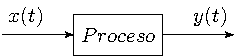
\includegraphics[width=0.5\textwidth]{esquemaLazoAbierto.pdf}
				\caption[Ejemplo de un sistema en lazo abierto]{\textbf{Sistema en lazo abierto}. Fuente: Elaboración propia.} 
				\label{fig:esquemaLazoAbierto}
            \end{figure}
        
        \subsubsection{Sistema en lazo cerrado}
		
			Los sistemas de lazo cerrado son aquellos cuya salida es realimentada a la entrada del sistema, esta realimentación suele ser negativa para que sea estable, no obstante, existen sistemas que se vuelven inestables con el simple hecho de cerrar el lazo, un ejemplo de sistema realimentado se puede observar en la \cref{fig:esquemaLazoCerrado}.
			
			\begin{figure}[htb]
				\centering
				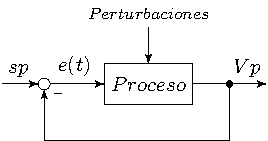
\includegraphics[width=0.6\textwidth]{esquemaLazoCerrado.pdf}
				\caption[Ejemplo de un sistema en lazo cerrado]{\textbf{Sistema en lazo cerrado}. Se observan las principales señales de un sistema en lazo cerrado. Fuente: Elaboración propia.} 
				\label{fig:esquemaLazoCerrado}
			\end{figure}
			
            En la \cref{fig:esquemaLazoCerrado} se denotan algunas de las señales que componen a un sistema de control, $sp$, que corresponde al set point o valor de referencia, $Vp$, que corresponde a la variable del proceso y es la variable a controlar, las perturbaciones, las cuales son magnitudes físicas que pueden afectar al proceso como la temperatura ambiente, presión, vibraciones, entre otras, y finalmente, $e(t)$, que corresponde a la señal de error la cual viene dada por la diferencia entre el valor de referencia y la variable medida \Parencite{maloney2006electronica}.
            
            \begin{equation}\label{eq:Serror}
				e(t) = sp - Vp
            \end{equation}
        
        \subsubsection{Lugar de las raíces}
            
            El lugar de las raíces es un método sencillo de diseño que se basa en conocer y manipular la ubicación de los polos del sistema en función de un parámetro de ganancia. Un ajuste en la ganancia puede provocar que los polos cambien de posicion en el plano complejo y se ubiquen en una posicion deseada o indeseada. \textcite{ogata2003ingenieria} considera que: \blockquote[p.270]{Al diseñar un sistema de control lineal, encontramos que el método del lugar de las raíces resulta muy útil, debido a que indica la forma en la que deben modificarse los polos y ceros en lazo abierto [...]}. En la \cref{fig:rootLocus} se observa un ejemplo de la grafica del lugar de las raices.

            \begin{figure}[htb]
                \centering
                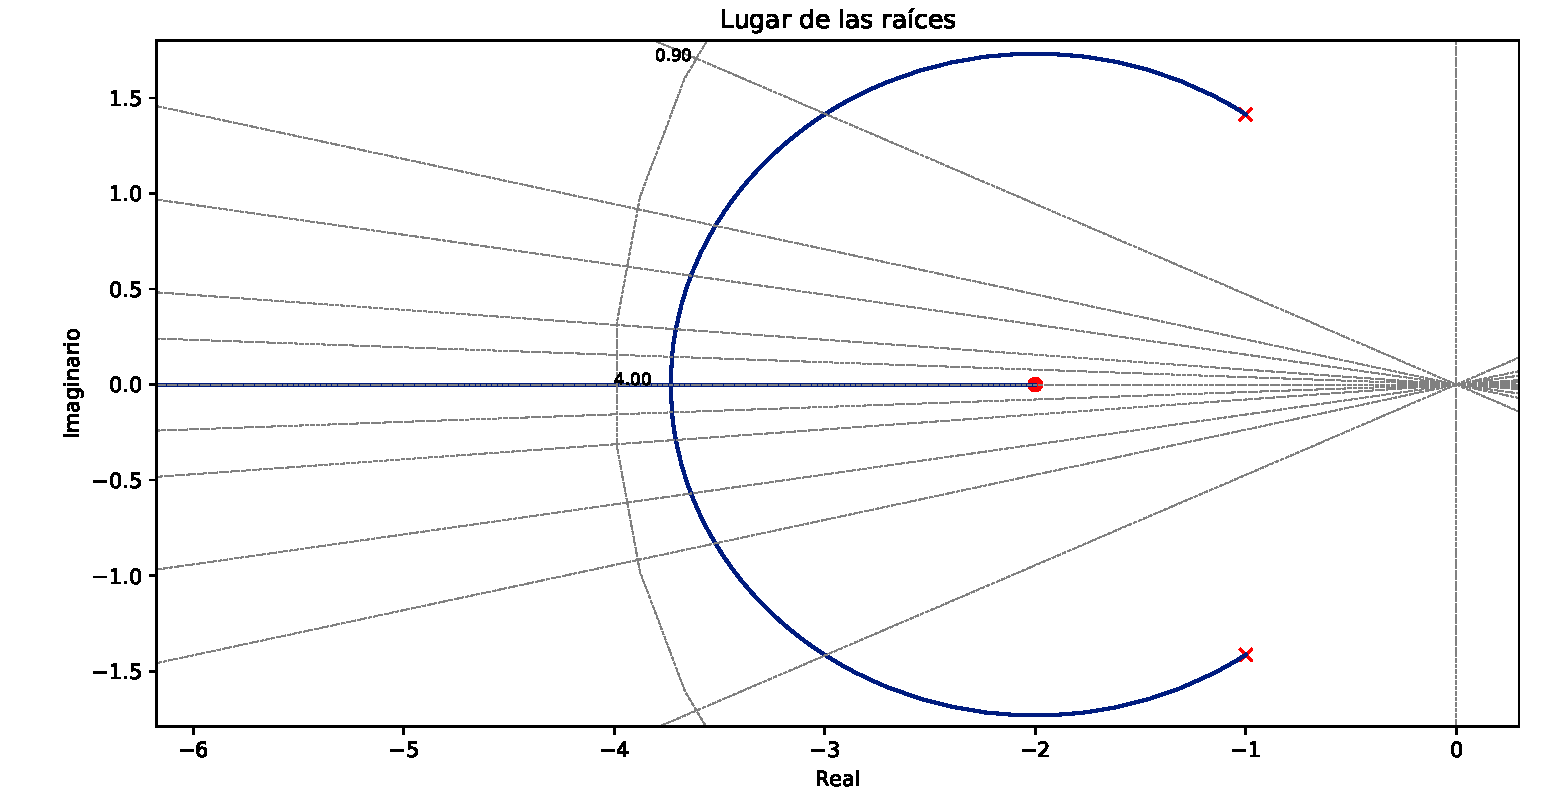
\includegraphics[width=0.75\textwidth]{rootLocus.pdf}
                \caption[Ejemplo de grafica del lugar de las raices]{\textbf{Grafica del lugar de las raices}. Se puede observar la grafica del lugar de las raices para un sistema $G_1(s) = \frac{s + 2}{s^2 + 2s + 3}$, el cual tiene ubicado sus polos en el semiplano izquierdo del plano complejo. Fuente: Elaboración propia.} 
                \label{fig:rootLocus}
            \end{figure}

        \subsubsection{Estabilidad de los sistemas}

            La estabilidad se ve afectada por la estructura del sistema, por tanto, se debe tomar en cuanta cuando se cierra el lazo del sistema. \textcite{ogata2003ingenieria} afirma que, desde el punto de vista de estabilidad, el sistema de control en lazo abierto no es un problema importante. Por otra parte, la estabilidad es un gran problema en el sistema de control en lazo cerrado debido a la posibilidad de que se generen oscilaciones. En consecuencia, los análisis de estabilidad se realizan para sistemas en lazo cerrado, el motivo principal es porque los sistemas en lazo abierto tienden a ser estables, además, para realizar el control de un proceso se suele utilizar los sistemas en lazo cerrado

            \paragraph{Análisis de estabilidad en el plano complejo}
            
                La estabilidad de un sistema lineal viene dada por la ubicación de sus polos a lo largo del plano complejo s, i.e., se puede determinar si un sistema es estable si no posee ninguno polo en el semiplano derecho del plano complejo s incluyendo el eje coordenado $j\omega$ en tiempo continuo \Parencite{ogata2003ingenieria}, en el caso de sistemas discretos, los polos deben encontrarse dentro del circulo unitario, la estabilidad marginal es posible si existen uno o mas polos justo en el circulo unitario, pero no multiples. El cual perimite que el análisis de estabilidad se puede realizar de forma analítica y gráfica. En la \cref{fig:pzmap} se puede observar dos sistemas continuos en lazo abierto, $G_1(s)$ que es estable y $G_2(s)$ que es inestable .

                \begin{figure}[htb]
                    \centering
                    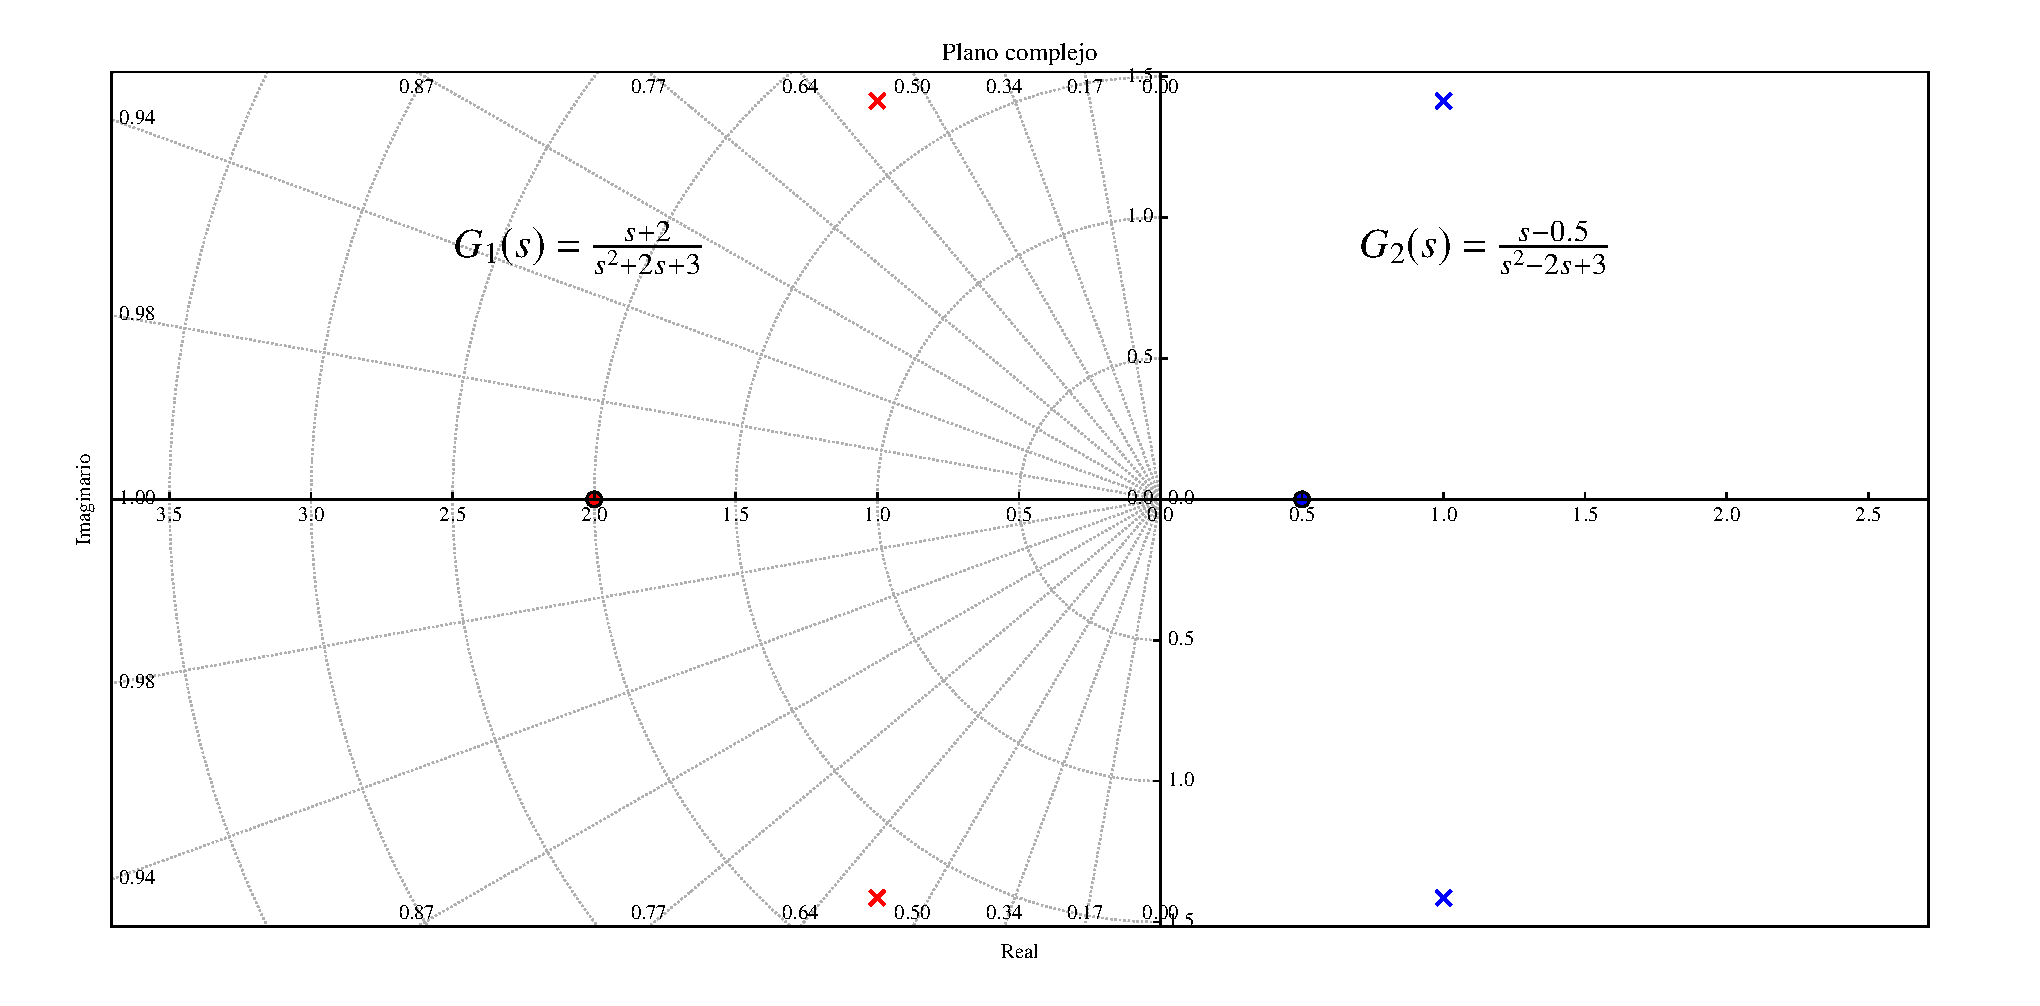
\includegraphics[width=0.8\textwidth]{pzmap.pdf}
                    \caption[Ejemplo de analisis de estabilidad en el plano complejo]{\textbf{Analisis de estabilidad en el plano complejo}. Se puede observar como el sistema $G_1(s)$ tiene ubicado sus polos en el semiplano izquierdo del plano complejo, i.e., es estable, por otro lado, el sistema $G_2(s)$ es inestable al poseer polos ubicados en el semiplano derecho del plano complejo. Fuente: Elaboración propia.} 
                    \label{fig:pzmap}
                \end{figure}
            
            \paragraph{Criterio de estabilidad de Nyquist}
                
                El criterio de estabilidad de Nyquist determina el estado de estabilidad utilizando los polos en lazo abierto y la respuesta en frecuencia del sistema en lazo abierto. Este criterio \enquote{es útil en la ingeniería de control, debido a que permite determinar gráficamente la estabilidad absoluta del sistema en lazo cerrado a partir de las curvas de respuesta en frecuencia en lazo abierto, sin que sea necesario determinar los polos en lazo cerrado}\Parencite[p.$\,$446]{ogata2003ingenieria}. Este criterio tiene la ventaja de poder realizarse tanto con cálculos analíticos como con datos experimentales, \textcite{ogata2003ingenieria} define tres criterios:

                \begin{enumerate}[leftmargin=\parindent]
                    \item El punto $-1 + j0$ no esta rodeado. Esto implica que el sistema es estable en lazo cerrado si no hay polos de $G(s)H(s)$ en el semiplano derecho del plano s\footref{fn:continuevsdiscreto}; de lo contrario, el sistema es inestable.
                    \item El punto $-1 + j0$ queda rodeado una o varias veces en sentido contrario al de las agujas
                    del reloj. En este caso, el sistema es estable en lazo cerrado si el número de rodeos en sentido contrario
                    al de las agujas del reloj es igual al número de polos $G(s)H(s)$ en el semiplano derecho
                    del plano s\footref{fn:continuevsdiscreto}; de lo contrario, el sistema es inestable.

                    \footnotetext[1]{En el caso de sistemas discretos se toma en cuenta son los polos fuera del circulo unitario para la evaluacion de los criterios. \label{fn:continuevsdiscreto}}

                    \item El punto $-1 + j0$ queda rodeado una o varias veces en el sentido de las agujas del reloj.
                    En este caso el sistema es inestable en lazo cerrado.
                \end{enumerate}
                
                En la \cref{fig:nyquistPlot} se puede observar los diagramas de Nyquist para los sistemas presentados en la \cref{fig:pzmap}, el sistema $G_1(s)$ debe ser evaluado por el criterio numero 1, al no poseer ninguno polo en el semiplano derecho el sistema sera estable en lazo cerrado asumiendo un $H(s) = 1$, por otro lado, $G_2(s)$ debe ser evaluado por el criterio numero 2, debido a que el numero de rodeos al punto $-1 + j0$ es igual al numero de polos en el semiplano derecho el sistema sera estable en lazo cerrado asumiendo un $H(s) = 1$ a pesar de que en lazo abierto sea inestable.

                \begin{figure}[htb]
                    \centering
                    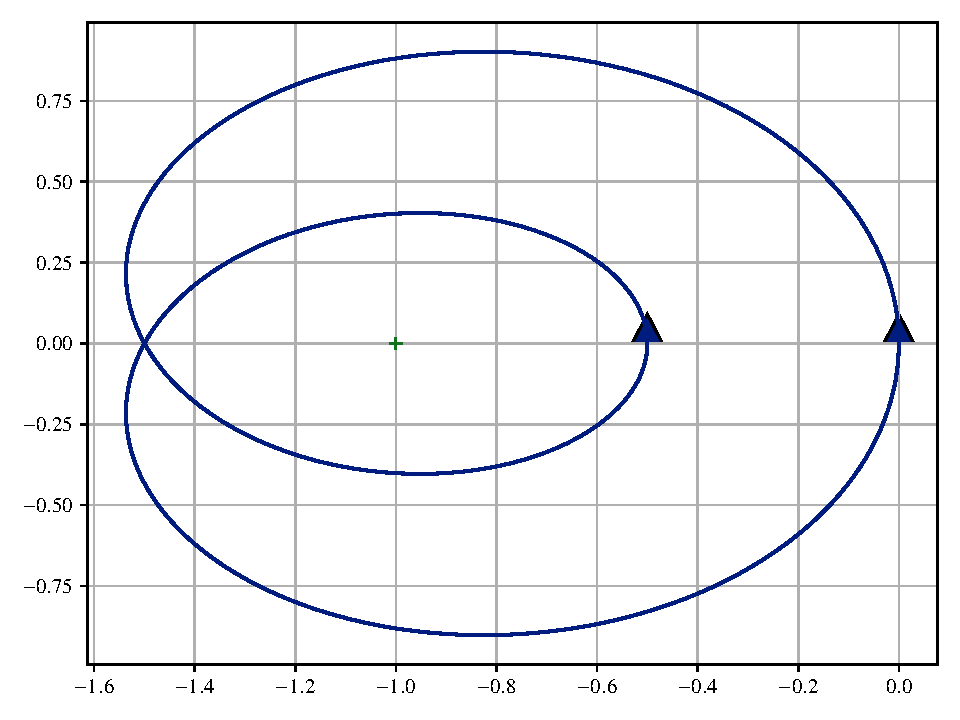
\includegraphics[width=0.7\textwidth]{nyquistPlot.pdf}
                    \caption[Ejemplo de analisis de estabilidad con diagrama de Nyquist]{\textbf{Analisis de estabilidad con diagrama de Nyquist}. El sistema $G_1(s)$ al ser evaluado con el criterio numero 1 se encuentra que es estable en lazo cerrado, a su vez, el sistema $G_2(s)$ al ser evaluado con el criterio numero 2 se encuentra que tambien sera estable en lazo cerrado, en ambos casos se asume un $H(s) = 1$. Fuente: Elaboración propia.} 
                    \label{fig:nyquistPlot}
                \end{figure}
            
            \paragraph{Margen de ganancia y Margen de fase}
                
                Los margenes de ganancia y de fase son una medida de la estabilidad relativa, se toman en cuenta a la hora de realizar el diseño de un controlador debido a que los margenes se pueden interpretar de modo que orienten en la cantidad de ganancia que se le puede aplicar al sistema en lazo cerrado, adicionalmente, la estabilidad relativa se puede interpretar como que tan estable es un sistema. \textcite{dorf2011modern} definen el margen de ganancia como: \blockquote[p.655]{[...] el incremento en la ganancia del sistema cuando $fase = -180^\circ$ que resultaria en un sistema marginalmente estable con la interseccion del punto $-1 + j0$ en el diagrama de Nyquist}. Asi mismo, \textcite{dorf2011modern} definen el margen de fase como: \blockquote[p.656]{[...] la cantidad de desplazamiento de fase de $L(j\omega)$ a una unidad de magnitud que resultaria en un sistema marginalmente estable con la intersección del punto $-1 + j0$ en el diagrama de Nyquist. El margen de ganancia y de fase pueden ser facilmente encontrados utilizando un diagrama de Bode.}

            \paragraph{Análisis de estabilidad con las trazas de Bode}

                Los diagramas de bode son una forma de representar la respuesta en frecuencia de un sistema tomando en cuenta los cambios de amplitud de $L(j\omega)$ y del ángulo de fase de $L(j\omega)$ respecto a la frecuencia \Parencite{nilsson1995circuitos}. Para analizar la estabilidad se utilizan el margen de ganancia y el margen de fase del sistema en un diagrama de Bode a modo de trazas, el punto de estabilidad critica en el diagrama de bode pasa a ser su equivalente en $dB$, el cual es $0dB$.

                Un margen de ganancia positivo y de fase positivos indican que el sistema es estable, si el sistema es de fase no minima, la interpretacion anterior deja de ser valida. Aplicando las deficiones dadas por \textcite{dorf2011modern} podemos obtener el margen de ganancia y de fase para los sistemas $G_1(s)$ y $G_2(s)$ y se presentan como ejemplo en la \cref{fig:bodeG1} y \cref{fig:bodeG2}.

                \begin{itemize}[leftmargin=\parindent]
                    \item $G_1(s)$: $GM \rightarrow \infty$ y $PM \rightarrow \infty$
                    \item $G_2(s)$: $GM = -3.509dB$ a $1.409\ rad/sec$ y $PM = -23.719^\circ$ a $0.807\ rad/sec$
                \end{itemize}

                \begin{figure}[htb]
                    \centering
                    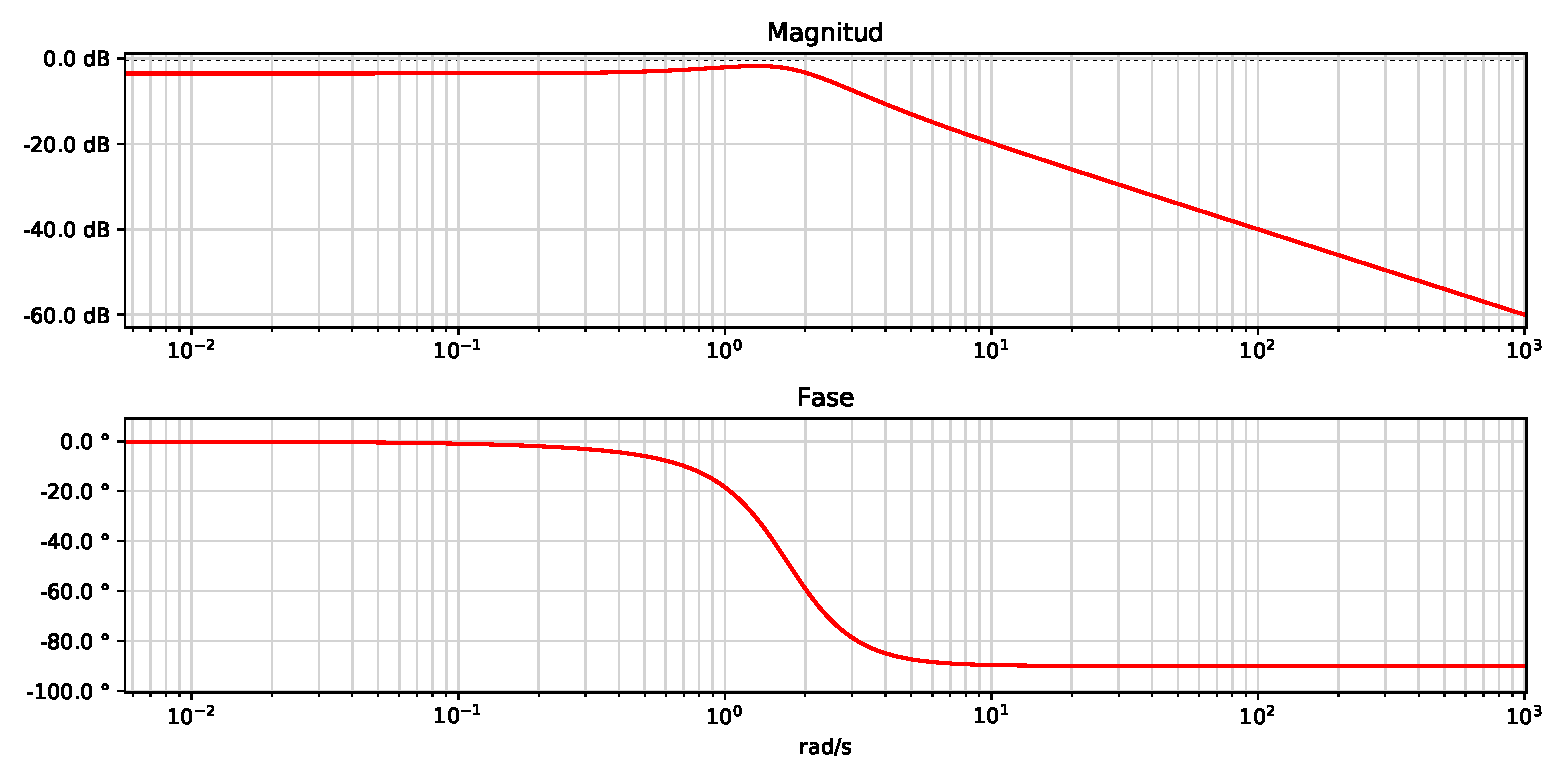
\includegraphics[width=\textwidth]{bodeG1.pdf}
                    \caption[Ejemplo 1 margenes de ganancia y fase]{\textbf{Margenes de ganancia y fase de $\pmb{G_1(s)}$}. En el diagrama se puede observar que no existe cruce por $0dB$ en magnitud o cruce por $-180^\circ$ en fase, por tanto, el sistema es estable y acepta incrementos teoricos de ganancia infinitos . Fuente: Elaboración propia.}
                    \label{fig:bodeG1}
                \end{figure}

                \begin{figure}[htb]
                    \centering
                    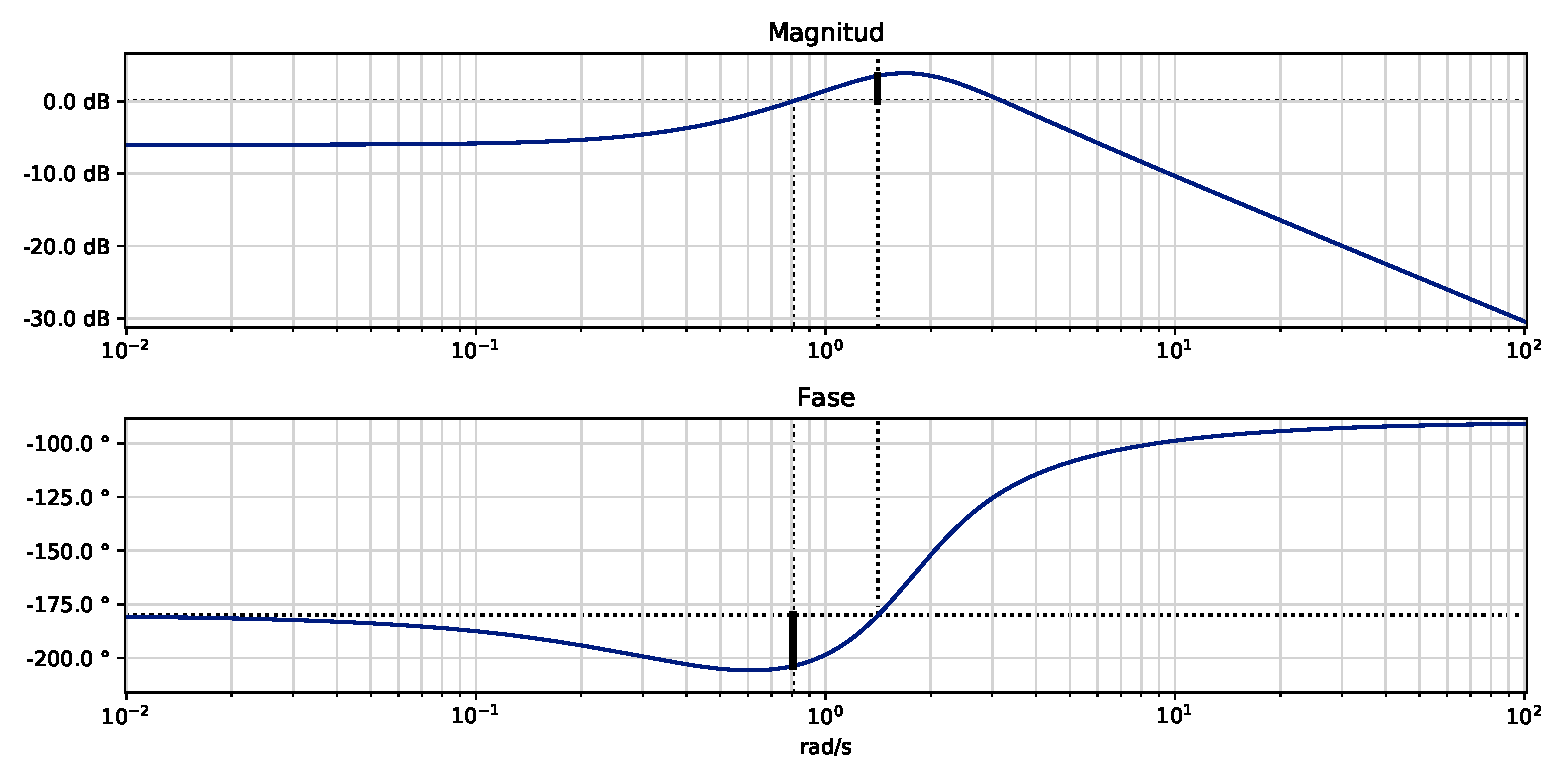
\includegraphics[width=\textwidth]{bodeG2.pdf}
                    \caption[Ejemplo 2 margenes de ganancia y fase]{\textbf{Margenes de ganancia y fase de $\pmb{G_2(s)}$}. El sistema $G_2(s)$ es de fase no minima, por tanto, la interpretacion del margen de ganancia y de fase no es tan simple. En la figura se observar que el margen de ganancia es negativo y aun asi, sabemos por su analisis con diagrama de Nyquist que es estable en lazo cerrado. Fuente: Elaboración propia.} 
                    \label{fig:bodeG2}
                \end{figure}

            \paragraph{Diagrama de Nichols}
                
                El diagrama de Nichols es una grafica del sistema en lazo abierto de tipo magnitud vs fase, en el diagrama se pueden ubicar los margenes de ganancia y fase, para ayudar en el diseño de controladores se suele superponer una rejilla guia de valores de magnitud y angulo constantes, esta rejilla lleva el nombre de carta de Nichols o abaco de Nichols. En el diagrama de nichols el punto critico $-1 + j0$ se convierte en $(0dB, -180^\circ)$

                \clearpage

        \subsubsection{Controlador PID}

            El controlador será el elemento dentro del sistema de control que se encargará de llevar al proceso a un valor de referencia deseado, existen varios esquemas de control para el control de procesos, cada uno con sus ventajas y desventajas, el más común es un sistema en lazo cerrado con controlador, este se puede observar en la \cref{fig:esquemaPID}.

            \begin{figure}[htb]
                \centering
                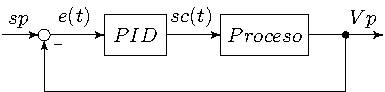
\includegraphics[width=\textwidth]{esquemaPID.pdf}
                \caption[Ejemplo de un sistema en lazo cerrado con controlador]{\textbf{Sistema en lazo cerrado con controlador}. El controlador recibe la señal de error y genera una señal de control $sc(t)$. Fuente: Elaboración propia.} 
                \label{fig:esquemaPID}
            \end{figure}

            En este esquema se observa que el controlador recibe la señal de error producto de tomar la diferencia entre el setpoint y la variable del proceso, este error es utilizado por el controlador para generar una señal de control $sc(t)$. El controlador más usado en la industria es el controlador PID, así lo afirma \textcite{kuo1996sistemas}: \enquote{[...] uno de los controladores más ampliamente empleados es el controlador PID [...] donde las letras son las iniciales de proporcional, integral y derivativo}(p.$\,$671). La ecuación que define a un PID en el dominio del tiempo es la siguiente:

            \begin{equation}\label{eq:pidtiempo}
                sc(t) = K_{p}e(t)+  K_{i}\int_{0}^{t} e(\tau) d\tau + K_{d} \frac{d}{dt}e(t)
            \end{equation}
            
            \noindent y su forma en función de transferencia:
            
            \begin{equation}\label{eq:pidcompleja}
                G_{c}(s) = \frac{sc(s)}{e(s)} = K_p + \frac{K_i}{s} + K_d s
            \end{equation}
            
            El controlador PID tambien puede ser representado de forma discreta, la componente proporcional sigue siendo una constante, la componente integral se puede representar como la sumatoria de todas las muestras multiplicadas por el periodo de muestreo y finalmente la derivada se puede aproximar como una diferencia finita regresiva:

            \begin{equation}\label{eq:pidcdiscreto}
                sc(k) = K_{p}e(k)+  K_{i}T\left[\sum_{i=0}^{k-1} e(i) + e(k)\right] + K_{d} \frac{e(k)- e(k-1)}{T}
            \end{equation}

            En el dominio Z, la componente proporcional se mantiene como constante, la componente integral puede ser aproximada con varios metodos numericos para el calculo de area como la integracion trapezoidal \Parencite{kuo1996sistemas}, o lo que es lo mismo, el metodo de Tustin, para el caso de la derivda se parte de su aproximacion como diferencia finita regresiva y se le aplica la transformada Z.

            \begin{equation}\label{eq:pidenZ}
                G_{c}(z) = K_{p} + \frac{K_{i}T}{2}\left(\frac{z+1}{z-1}\right) + K_{d} \frac{z-1}{Tz}
            \end{equation}

            \paragraph{Componente proporcional}

				La componente proporcional se obtiene de multiplicar la señal de error por la ganancia proporcional, lo cual provoca que la señal de control sea proporcional a la señal de error con una relación igual a la ganancia proporcional, si el controlador solo constase de componente proporcional el error en estado estable nunca se eliminaría, dicho de otro modo, el error podría ser muy bajo, pero jamás cero. \enquote{Este error se denomina la desviación permanente u \enquote{offset}. El mismo disminuye si se aumenta el valor de K}\Parencite[p.$\,$54]{nelson1999fundamentos}.

			\paragraph{Componente integral}

				La componente integral viene dada por la sumatoria de la señal del error en el tiempo multiplicada por la ganancia integral, por tanto, se obtiene una acumulación en un periodo determinado, lo anterior implica que mientras exista error, la componente integral seguirá aumentando o disminuyendo dependiendo del signo de la señal de error hasta que el error sea cero, la componente integral se suma con la componente proporcional formando una única señal de control.

				Debido a que la componente integral depende del tiempo, es posible corregir desviaciones de la variable controlada generadas por perturbaciones externas. Por otro lado, debido a que eventualmente se conseguirá que el error sea igual a cero la componente proporcional no hará ningún aporte al sistema, y la señal de control pasará a ser totalmente generada por la componente integral hasta que exista un cambio en el setpoint o una alteración en la variable medida.

			\paragraph{Componente derivativa}

				La componente derivativa viene dada por el ritmo de cambio de la señal de error multiplicado por la ganancia derivativa, por tanto, cuando el error permanece constante la componente derivativa es igual a cero, la componente derivativa será tan grande como la velocidad con la que cambie el error, lo cual ayuda a evitar que se generen sobre pasos en la variable medida respecto a la variable de referencia.
				
				La componente derivativa es muy sensible al ruido, por tanto, se debe utilizar solo cuando se requiera un cierto grado de anticipación y no exista ruido \Parencite{smith1985principles}. Es recomendable utilizar filtros en orden de disminuir el posible ruido, a su vez, cuando el proceso a controlar es de respuesta rápida se recomienda no agregar componente derivativa o que su ganancia sea muy pequeña. Tomando en cuenta lo anterior, se debe mencionar que la componente derivativa tal como se observa en las ecuaciones \cref{eq:pidtiempo} y \cref{eq:pidcompleja} no es implementable al ser no causal, por tanto, la derivada puede ser implementada utilizando una aproximacion. \blockquote[{\cite[p.220]{aastrom2002control}}]{La aproximacion actua como una derivada para las componentes de la señal de baja frecuencia. La ganancia, sin embargo, esta limitada a $KN$. Esto significa que las medidas de ruido de alta frecuencia son amplificados cuando mucho por un factor $KN$.} La funcion de transferencia de la componente derivativa aproximada es la siguiente:

                \begin{equation}\label{eq:Daproximacion}
                    D = K_d \frac{N s}{s + N}
                \end{equation}

        \subsubsection{Entonación por método de Ziegler-Nichols en lazo abierto}
			
            El método de Ziegler-Nichols en lazo abierto requiere primero aproximar el modelo del proceso como una función de transferencia de primer orden con tiempo muerto.
            
            \begin{equation}\label{eq:firstorderProcess}
                G(s) = \frac{K}{\tau s + 1} e^{-\alpha s}
            \end{equation}
            
            Los parámetros correspondientes pueden ser obtenidos realizando una prueba al escalón y extrayendo los datos correspondientes de la gráfica de la respuesta, un ejemplo se puede observar en la \cref{fig:ZNtest}. Acá se observa: (a) $t_{0}$ que corresponde al inicio del escalón, (b) $t_{1}$ inicio de la respuesta por parte del proceso al escalón, (c) $t_{2}$ cuando el proceso alcanza el 63\% del cambio total, (d) $\Delta y$ cambio total del proceso ante el escalón y (e) $\Delta u$ magnitud de cambio de la entrada. Los parámetros para aproximar el proceso a un modelo de primer orden con tiempo muerto se calculan como sigue:
            
            \begin{align}\label{eq:parametros}
                K &= \frac{\Delta y}{\Delta u}\\
                \tau &= t_{2} - t_{1}\\
                \alpha &= t_{1} - t_{0}
            \end{align}
            
            \begin{figure}[htb]
                \centering
                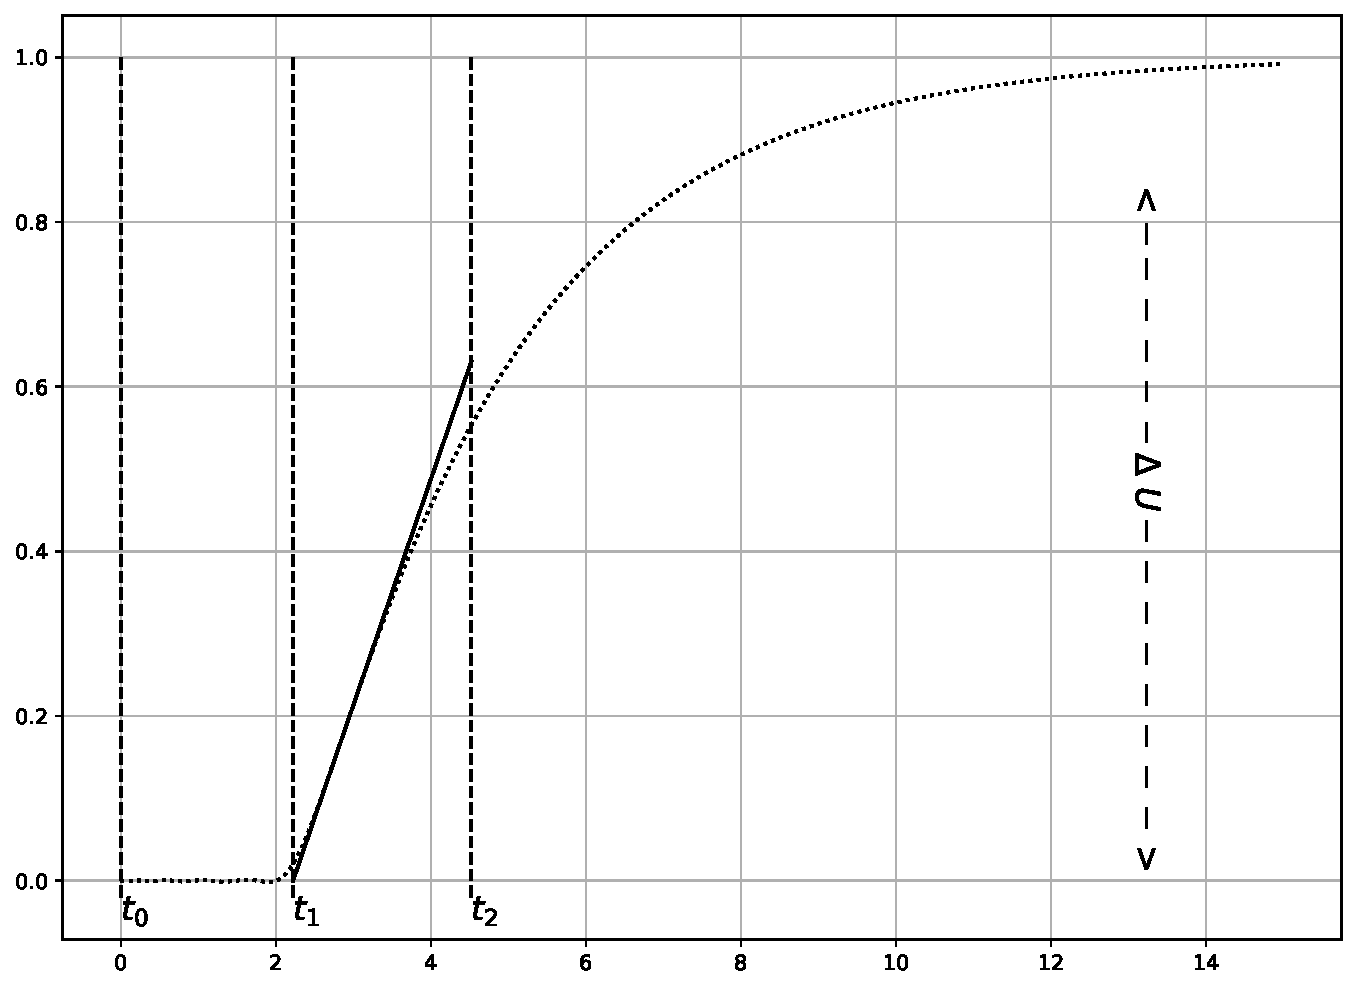
\includegraphics[width=0.9\textwidth]{ZieglerN.pdf}
                \caption[Modelado por curva de reacción]{\textbf{Modelado por curva de reacción.} Para realizar este modelado se estudia la respuesta del sistema ante la entrada de la función de heaviside u(t), también llamada función escalón unitario, el modelo obtenido a través de este método es una aproximación del sistema. Fuente: Elaboración propia.} 
                \label{fig:ZNtest}
            \end{figure}
            
            Con los parametros del modelo de primer orden se puede obtener la entonación de un controlador P, PI o PID. Las ganancias $K_{p}$, $K_{i}$ y $K_{d}$ se pueden obtener sustituyendo los mencionados parametros en la \cref{tab:ZiglerNichols} correspondiente a la regla de entonación de Ziegler-Nichols. \textcite{ogata2003ingenieria} comenta que: \enquote{Las reglas de sintonía de Ziegler-Nichols [...] se han usado ampliamente para sintonizar controladores PID en sistemas de control de procesos en los que no se conoce con precisión la dinámica de la planta}(p.$\,$572).
            
            \begin{table}[htb]
                \centering
                \begin{threeparttable}
                    \renewcommand{\arraystretch}{1.5} 	% Separacion de las filas
                    %\setlength{\tabcolsep}{6pt}			% Separacion de columnas
                    \caption[Regla de entonación de Zigler-Nichols]{Regla de entonación de Zigler-Nichols}
                    \begin{tabular*}{\textwidth}{c @{\extracolsep{\fill}}ccc}
                        \toprule
                        Tipo de controlador & $K_{p}$                               &              $T_{i}$              &         $T_{d}$          \\ \midrule
                                    P          & $\displaystyle\frac{\tau}{\alpha}$    &       $\displaystyle\infty$       &            0             \\[20pt]
                                PI          & $0.9\displaystyle\frac{\tau}{\alpha}$ & $\displaystyle\frac{\alpha}{0.3}$ &            0             \\[20pt]
                                PID         & $1.2\displaystyle\frac{\tau}{\alpha}$ &      $2\displaystyle\alpha$       & $0.5\displaystyle\alpha$ \\ \bottomrule
                    \end{tabular*}
                    \label{tab:ZiglerNichols}
                    \begin{tablenotes}[flushleft]
                        \item {\footnotesize \textbf{Nota.} Los valores de $K_{i}$ y $K_{d}$ se pueden obtener de la siguiente forma: $K_{i} = K_{p}/T_{i}$ ; $K_{d} = K_{p}T_{d}$. Fuente: \textcite{ogata2003ingenieria}.}
                    \end{tablenotes}
                \end{threeparttable}
            \end{table}
            
            Adicionalmente existen otras reglas para la entonacion automatica de los controladore PID, como el metodo de Cohen-Coon, al igual que Ziegler-Nichols, requiere de los parametros del proceso en su aproximacion como proceso de primer orden para ser sustituidos en la \cref{tab:CohenCoon} y obtener las ganancias respectivas.
            
            \clearpage

            \begin{table}[htb]
                \centering
                \begin{threeparttable}
                    \renewcommand{\arraystretch}{1.5} 	% Separacion de las filas
                    %\setlength{\tabcolsep}{6pt}			% Separacion de columnas
                    \caption[Regla de entonación de Cohen-Coon]{Regla de entonación de Cohen-Coon}
                    \begin{tabular*}{\textwidth}{c @{\extracolsep{\fill}}ccc}
                        \toprule
                        Tipo de controlador & $K_{p}$                               &              $T_{i}$              &         $T_{d}$          \\ \midrule \renewcommand{\arraystretch}{3.5}
                                    P          & $\displaystyle\frac{1}{K}\left(\displaystyle\frac{\tau}{\alpha}\right)\left[1 + \displaystyle\frac{1}{3}\left(\displaystyle\frac{\alpha}{\tau} \right) \right]$    &       $\displaystyle\infty$       &            0             \\[25pt]
                                PI          & $\displaystyle\frac{1}{K}\left(\displaystyle\frac{\tau}{\alpha}\right)\left[0.9 + \displaystyle\frac{1}{12}\left(\displaystyle\frac{\alpha}{\tau} \right) \right]$ & $\alpha\left[ \displaystyle\frac{30 + 3\left(\displaystyle\frac{\alpha}{\tau} \right) }{9 + 20\left(\displaystyle\frac{\alpha}{\tau} \right) } \right]$ &            0             \\[25pt]
                                PD & $\displaystyle\frac{1}{K}\left(\displaystyle\frac{\tau}{\alpha}\right)\left[\displaystyle\frac{5}{4} + \displaystyle\frac{1}{6}\left(\displaystyle\frac{\alpha}{\tau} \right) \right]$ & $\displaystyle\infty$ & $\alpha\left[ \displaystyle\frac{6 - 2\left(\displaystyle\frac{\alpha}{\tau} \right) }{22 + 3\left(\displaystyle\frac{\alpha}{\tau} \right) } \right]$ \\[25pt]
                                PID         & $\displaystyle\frac{1}{K}\left(\displaystyle\frac{\tau}{\alpha}\right)\left[\displaystyle\frac{4}{3} + \displaystyle\frac{1}{4}\left(\displaystyle\frac{\alpha}{\tau} \right) \right]$ &      $\alpha\left[ \displaystyle\frac{33 + 6\left(\displaystyle\frac{\alpha}{\tau} \right) }{13 + 8\left(\displaystyle\frac{\alpha}{\tau} \right) } \right]$       & $\alpha\left[ \displaystyle\frac{4}{11 + 2\left(\displaystyle\frac{\alpha}{\tau} \right) } \right]$ \\ \bottomrule
                    \end{tabular*}
                    \label{tab:CohenCoon}
                    \begin{tablenotes}[flushleft]
                        \item {\footnotesize \textbf{Nota.} Los valores de $K_{i}$ y $K_{d}$ se pueden obtener de la siguiente forma: $K_{i} = K_{p}/T_{i}$ ; $K_{d} = K_{p}T_{d}$. Fuente: \textcite{apcoCC}.}
                    \end{tablenotes}
                \end{threeparttable}
            \end{table}

    \subsection{Lógica difusa}
    
        La lógica difusa es una extensión matemática de la lógica convencional en donde se asigna un grado de pertenencia a un hecho entre un valor verdadero y uno falso, \enquote{consiste en que los valores verdaderos (en lógica difusa) o valores de pertenencia (en conjuntos difusos) se indican en un número entre [0.0, 1.0], donde 0.0 representa falsedad total y 1.0 significa verdad absoluta}\Parencite[p.$\,$4]{cruz2010inteligencia}.
        
        La lógica difusa se puede estructurar en tres etapas, la primera etapa consiste en establecer cada una de las variables con etiquetas lingüística que determinen en conjunto el universo de discurso de cada una de ellas, es decir, se crean los conjuntos difusos, en la segunda etapa se definen las reglas de inferencia difusa que determinaran el comportamiento del sistema difuso, y tercera, se obtienen los valores de salida utilizando las reglas de inferencia y realizando el proceso de defuzzificación que consiste en llevar los grados de pertenencia a un valor nítido o real \Parencite{cruz2010inteligencia}. 
        
        \subsubsection{Conjuntos difusos}
            
            Un conjunto difuso está compuesto de funciones de membresía, dichas funciones de membresía representan valores para asignar el grado de pertenencia de una variable a un estado en particular y son identificados con etiquetas lingüísticas descriptivas, como alto, caliente, bajo, negativo, entre otras. En la \cref{fig:FuzzySet} se puede observar un ejemplo de conjunto difuso.
            
            \begin{figure}[htb]
                \centering
                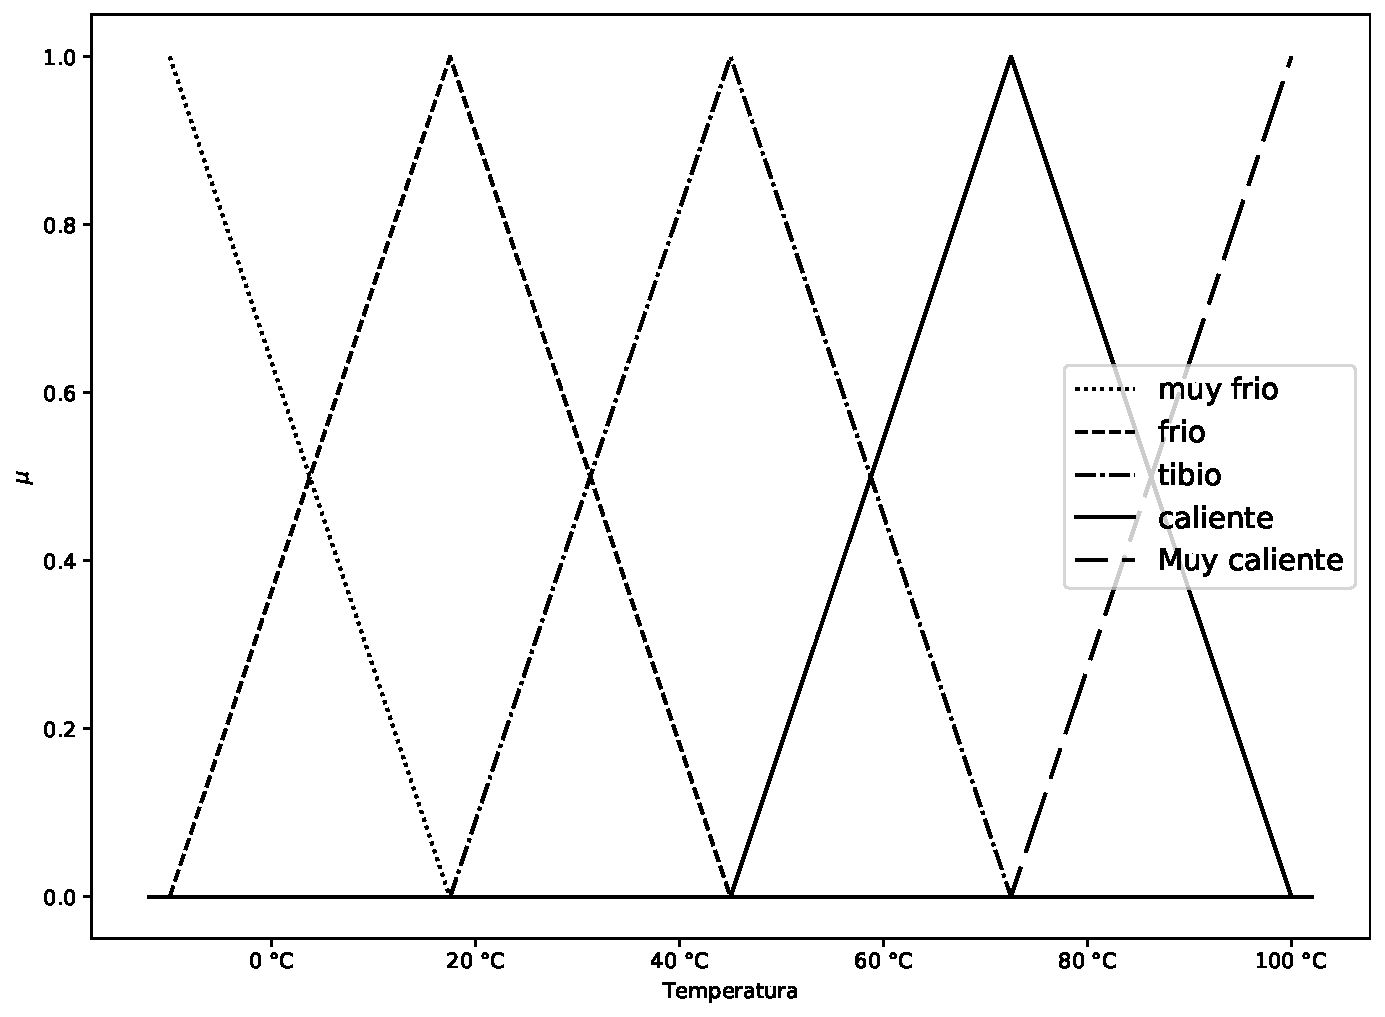
\includegraphics[width=0.7\textwidth]{FuzzySet.pdf}
                \caption[Ejemplo de un conjunto difuso]{\textbf{Ejemplo de un conjunto difuso}. Este conjunto difuso corresponde a una variable de temperatura que va desde -10\textdegree C hasta 100\textdegree C. Fuente: Elaboración propia.} 
                \label{fig:FuzzySet}
            \end{figure}
            
            Las funciones de membresía pueden tomar varias formas y rangos en orden de poder representar de mejor forma los grados de pertenencia de la variable a una etiqueta en particular, sin embargo, las formas triangulares suelen ser las menos pesadas en memoria y en poder de cómputo \Parencite{riid2003transparent}. La cantidad de etiquetas que se pueden asignar a un conjunto difuso es ilimitada, pero se debe tener en cuenta el nivel de complejidad que se genera a medida que se incrementa su número. A continuacion se muestran algunas formas que pueden tomar las funciones de membresia:

            \paragraph{Funcion de membresia: triangular o trimf}$\quad$
            
            \begin{equation*}\label{eq:trimf}
                \mu_n(x) = \left\{
                    \begin{aligned}
                        &\quad 0  &\quad &Si \quad & x &\leq a\\
                        &\frac{x - a}{b - a}  &\quad &Si \quad &  a \le &x \leq b \\
                        &\frac{c - x}{c - b}  &\quad &Si \quad & b \le &x \leq c \\
                        &\quad 0  &\quad &Si \quad&  x &\geq c
                    \end{aligned}\right.
                    \qquad
                    \raisebox{-15mm}{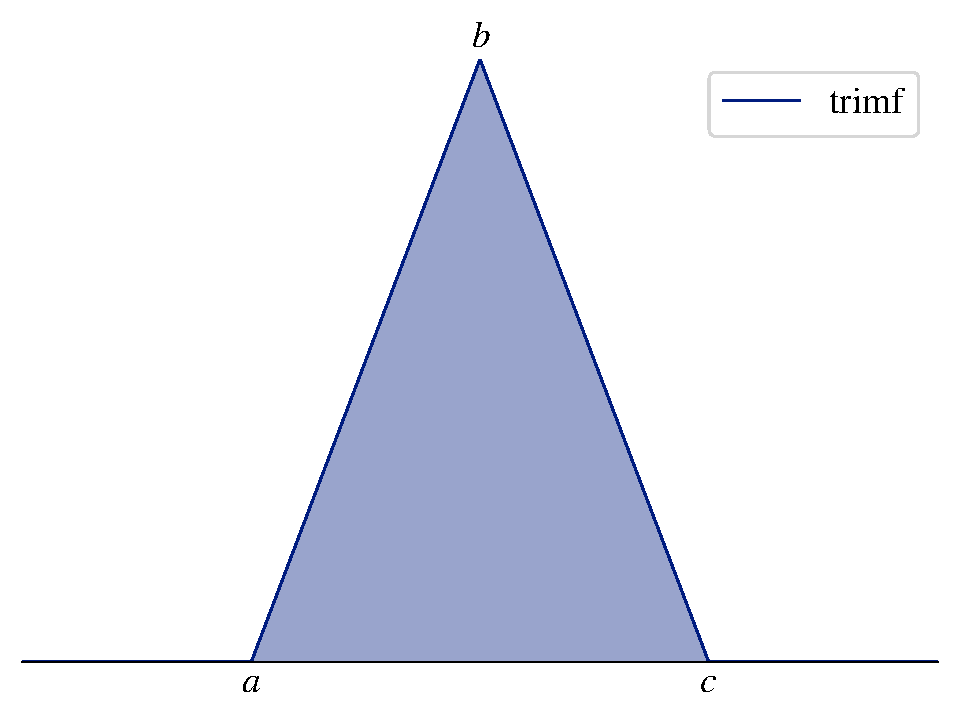
\includegraphics[width=0.28\linewidth]{trimf.pdf}}
            \end{equation*}
            
            \paragraph{Funcion de membresia: trapezoidal o trapmf}$\quad$
            
                \begin{equation*}\label{eq:trapmf}
                    \mu_n(x) = \left\{
                        \begin{aligned}
                            &\quad 0  &\quad &Si \quad &  x &\leq a\\
                            &\frac{x - a}{b - a}  &\quad &Si \quad &  a \le &x \leq b \\
                            &\quad 1 &\quad &Si \quad &  b \le &x \leq c \\
                            &\frac{d - x}{d - c}  &\quad &Si \quad & c \le &x \leq d \\
                            &\quad 0  &\quad &Si \quad & x &\geq d
                        \end{aligned}\right.
                        \qquad
                        \raisebox{-15mm}{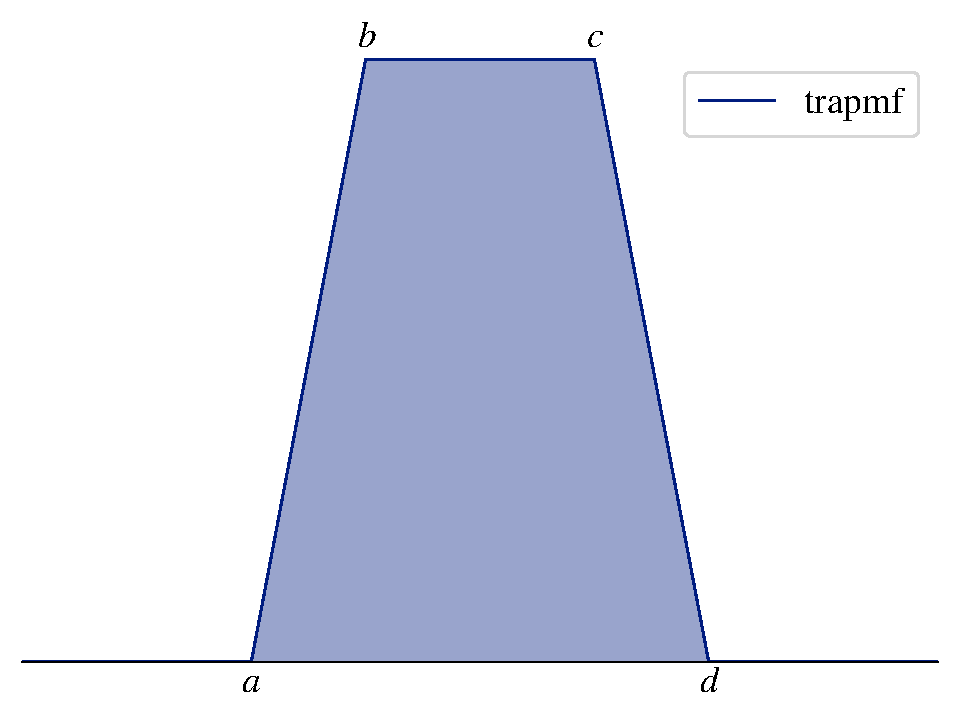
\includegraphics[width=0.28\linewidth]{trapmf.pdf}}
                \end{equation*}

            \paragraph{Funcion de membresia: gaussiana o gaussmf}$\quad$
                
                \begin{equation*}\label{eq:gaussmf}
                    \mu_n(x) = e^{-\frac{(x-m)^2}{2\sigma^2}}
                        \qquad \qquad
                        \raisebox{-15mm}{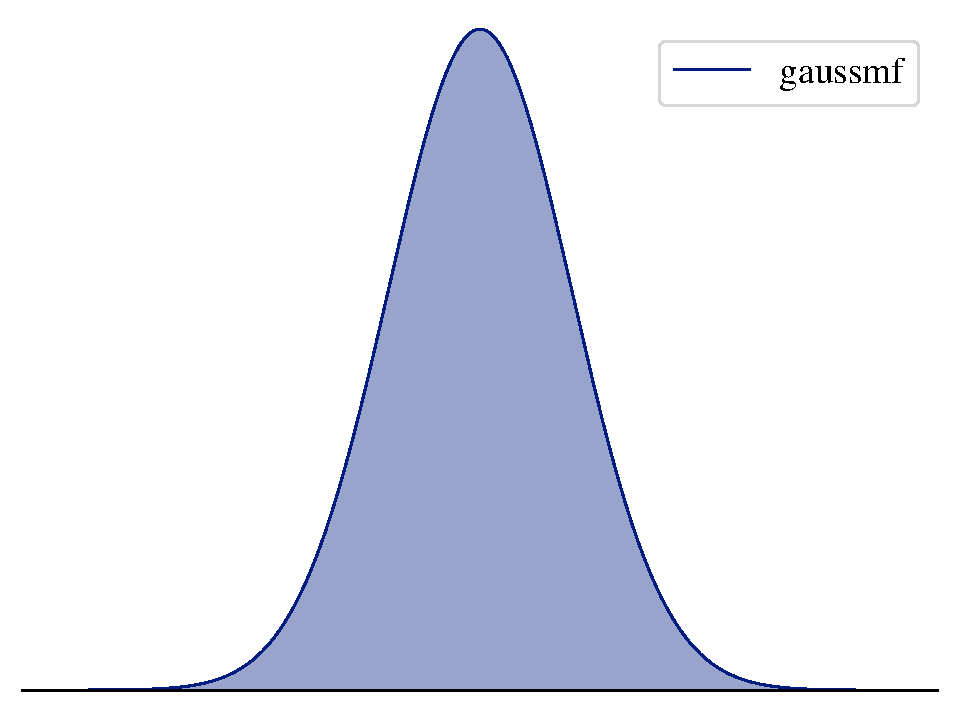
\includegraphics[width=0.28\linewidth]{gaussmf.pdf}}
                \end{equation*}
                
            \paragraph{Funcion de membresia: S o smf}$\quad$
                
                \begin{equation*}\label{eq:smf}
                    \mu_n(x) = \left\{
                        \begin{aligned}
                            &\quad 0  &\quad &Si \quad & x &\leq a\\
                            &2\left(\frac{x - a}{b - a}\right)^2  &\quad &Si \quad &  a \leq &x \leq \frac{a+b}{2} \\
                            &1 - 2\left(\frac{x - b}{b - a}\right)^2  &\quad &Si \quad & \frac{a+b}{2} \leq &x \leq b \\
                            &\quad 1  &\quad &Si \quad & x &\geq b
                        \end{aligned}\right.
                        \qquad
                        \raisebox{-15mm}{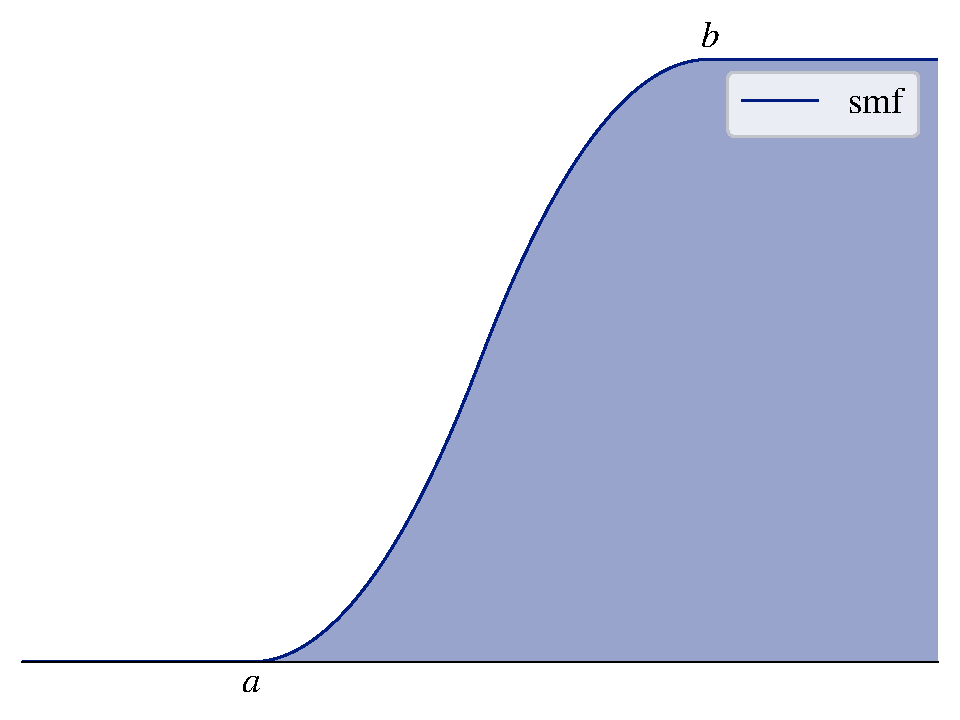
\includegraphics[width=0.28\linewidth]{smf.pdf}}
                \end{equation*}
            
            \paragraph{Funcion de membresia: Z o zmf}$\quad$
                
                \begin{equation*}\label{eq:zmf}
                    \mu_n(x) = \left\{
                        \begin{aligned}
                            &\quad 1  &\quad &Si \quad & x &\leq a\\
                            &1 - 2\left(\frac{x - a}{b - a}\right)^2  &\quad &Si \quad &  a \leq &x \leq \frac{a+b}{2} \\
                            &2\left(\frac{x - b}{b - a}\right)^2  &\quad &Si \quad & \frac{a+b}{2} \leq &x \leq b \\
                            &\quad 0  &\quad &Si \quad & x &\geq b
                        \end{aligned}\right.
                        \qquad
                        \raisebox{-15mm}{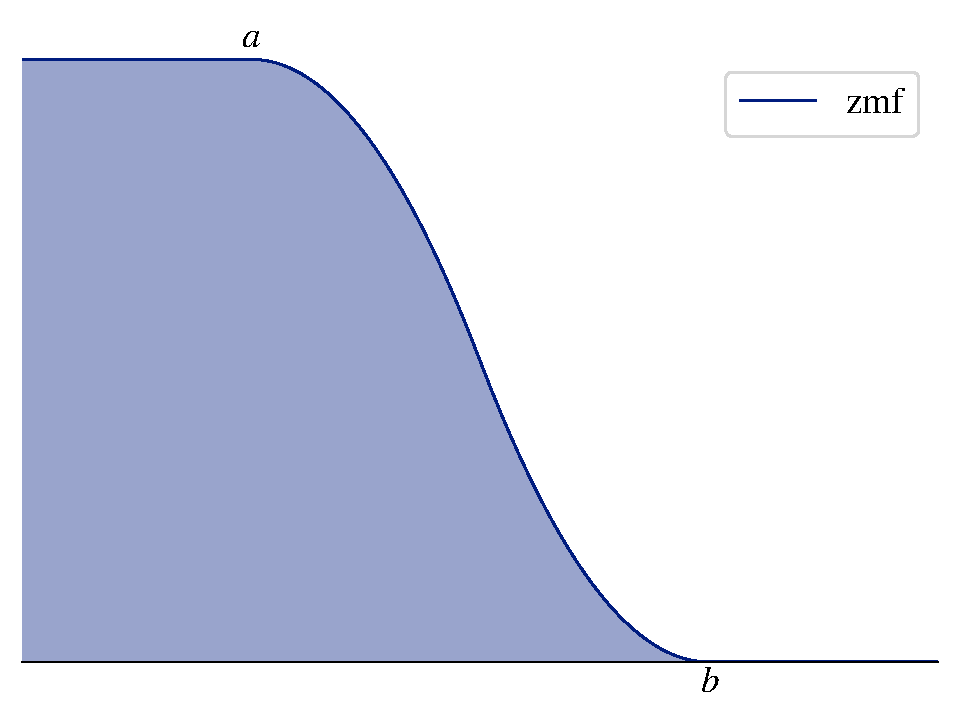
\includegraphics[width=0.28\linewidth]{zmf.pdf}}
                \end{equation*}

            \paragraph{Funcion de membresia: sigmoidal o sigmf}$\quad$
                
                \begin{equation*}\label{eq:sigmf}
                    \mu_n(x) = \frac{1}{1+e^{-c(x-b)}}
                        \qquad \qquad
                        \raisebox{-15mm}{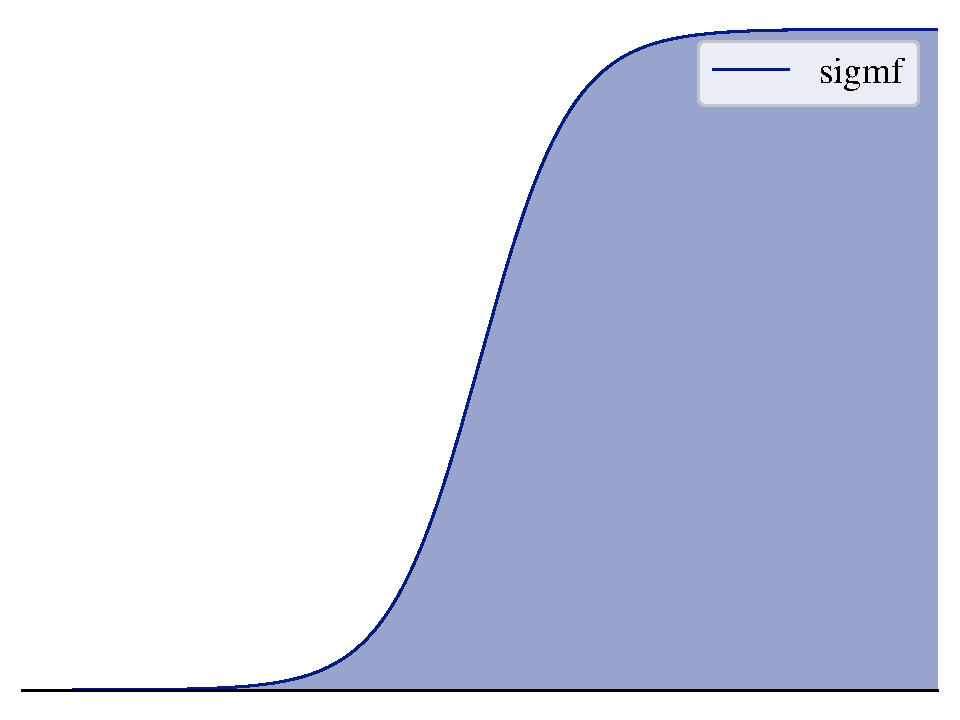
\includegraphics[width=0.28\linewidth]{sigmf.pdf}}
                \end{equation*}
               
            \paragraph{Funcion de membresia: campana generalizada o gbellmf}$\quad$
                
                \begin{equation*}\label{eq:gbellmf}
                    \mu_n(x) = \frac{1}{1+ \left|\frac{x - c}{a}\right|^{2b}}
                        \qquad \qquad
                        \raisebox{-15mm}{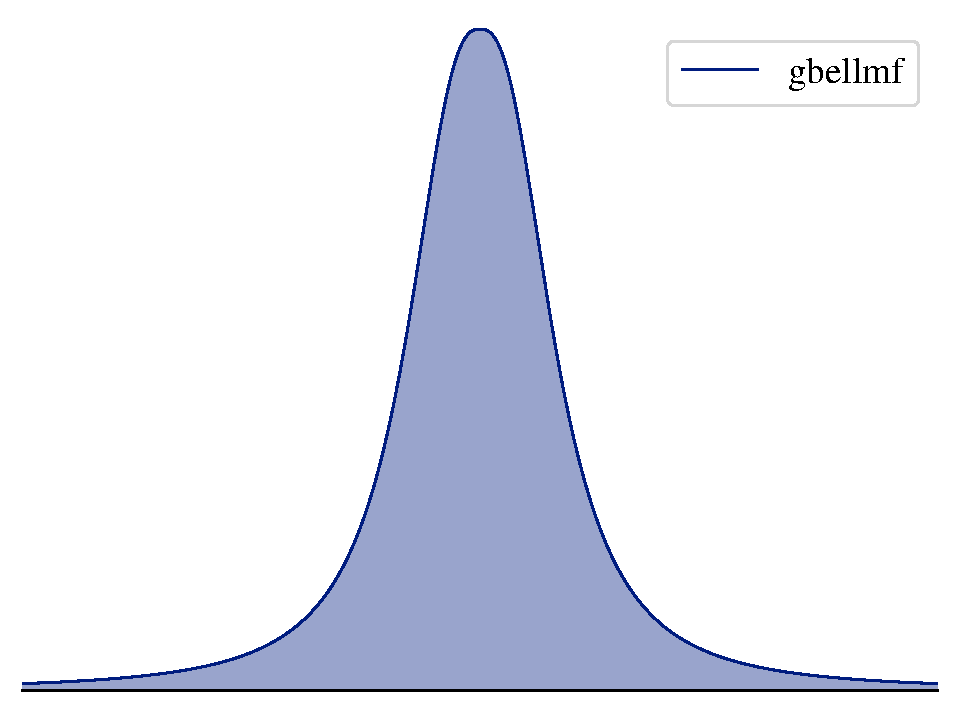
\includegraphics[width=0.28\linewidth]{gbellmf.pdf}}
                \end{equation*}

            Existen otras funciones de membresian que utilizan como base las anteriores mostradas, estas son:

            \begin{itemize}[leftmargin=\parindent]
                \item gauss2mf: Combinacion de dos funciones gaussianas.
                \item dsigmf: Valor absoluto de la diferencia de dos funciones sigmoidales.
                \item psigmf: Producto de dos funciones sigmoidales.
                \item pimf: Producto de una smf y una zmf.
            \end{itemize}
        
        \subsubsection{Reglas de inferencia}
            
            Las reglas de inferencia, al igual que en la lógica convencional, se encargan de realizar una conexión entre los antecedentes y los consecuentes con el fin de obtener una salida, en este caso, entre los conjuntos difusos de entrada y la salida, la cual puede ser un conjunto difuso o una función matemática. Como sugiere \textcite{cruz2010inteligencia}, las reglas pueden formularse de dos formas denominadas modus ponens y modus tollens. Modus ponens utiliza los antecedentes para obtener el consecuente, por otro lado, el modus tollens utiliza los consecuentes recíprocos para obtener el antecedente.
                        
            Para realizar el proceso de inferencia se necesitan las normas triangulares (T-Normas) para el caso de logica AND o las conormas triangulares (T-Conormas) para logica OR. Sus formas de aplicacion mas comunes suelen ser el minimo de los valores de pertenencia para las T-Normas y el maximo de los valores de pertenencia para las T-Conormas, de este modo, se obtienen las operaciones de interseccion y union respectivamente. El proceso de inferencia consta de 6 pasos: fuzzificacion, pareo de proposiciones,  conjuncion/disyuncion de premisas, implicacion, agregacion y defuzzificación.
        
        \subsubsection{Fuzzificacion}
            
            El proceso de fuzzificacion es el primer paso para obtener la salida de un controlador difuso. La entrada nitida es transformada en una representacion difusa, esto se debe a que las operaciones subsiguientes se realizan entre conjuntos difusos. La forma mas comun de fuzzificacion para la entrada es el uso de un singleton.
            
        \subsubsection{Pareo de proposiciones}
            
            \textcite{riid2003transparent} sugiere que en orden de evaluar la proposicion de premisas en terminos numericos los valores de membresia $\mu_{ir}$ respecto a x deben ser hayados para poder realizar el pareo de proposiciones. El pareo de proposiciones es la relacion que existe entre la entrada y una etiqueta lingüística. \textcite{riid2003transparent} afirma que \blockquote[p.16]{[...] el singleton difuso puede considerarse solo una representación diferente de un número nítido, por lo tanto, con fuzzificación singleton, el procedimiento de fuzzificación es incrustado en el pareo de proposiciones}. Utilizando fuzzificacion singleton el pareo de proposiciones puede representarse como:

            \begin{equation}\label{eq:preposiciones}
                \tau_{ir} = \mu_{ir}(x_i)
            \end{equation}

            \noindent donde i es la i-esima entrada al controlador difuso y r es la r-esima regla.
            
        \subsubsection{Operacion de premisas}
            
            Debido a que pueden existir N entradas, tambien pueden existir N premisas en una regla, las cuales, pueden relacionarce entre si por medio de operaicones AND en cuyo caso se denomina conjuncion de premisas. Por otro lado, tambien es posible relacionar las premisas utilizando las operaciones OR y se denomina disyuncion de premisas. Para realizar estas operaciones se pueden utilizar las T-Normas y las T-Conormas en el caso conjuncion y disyuncion respectivamente.

            \begin{align}
                &\text{Conjuncion de premisas:} & \tau_{r} &= \bigcap_{i=1}^{N}\tau_{ir} \label{eq:conjP} \\
                &\text{Disyuncion de premisas:} & \tau_{r} &= \bigcup_{i=1}^{N}\tau_{ir} \label{eq:disyP}
            \end{align}

        \subsubsection{Implicacion}

            La implicacion se encarga de relacionar las premisas con los concecuentes. Normalmente se prefiere utilizar conjuncion por medio de las T-Normas para realizar la implicacion, la cual viene descrita como sigue:

            \begin{equation}\label{eq:implicacion}
                F_r(y) = W_r \tau_{r} \cap \gamma_r
            \end{equation}

            \noindent donde $\gamma_r$ es la salida de la funcion de membresia asociada con la $r$-esima regla y $W_r$ es el peso asociado a la r-esima regla \Parencite{riid2003transparent}.

        \subsubsection{Agregacion}

            El proceso de agregacion se realiza luego de haber pasado por la fuzzificacion, pareo de proposiciones, conjuncion/disyuncion de premisas y la implicacion. Todos los resultados obtenidos de cada una de las reglas son unificados aplicando un operador OR por medio de una T-Conorma, de este modo, se obtiene un conjunto difuso por cada salida del controlador. Todo el proceso hasta este punto puede ser descrito por las siguientes formulas:

            \vspace{10pt}
            \begin{align}
                &\text{Con conjuncion de premisas:} & F(y) &= \bigcup_{r=1}^{R}\left(W_r \left(\bigcap_{i=1}^{N}\mu_{ir}(x_i) \right) \cap \gamma_r\right) \label{eq:fconjuncion} \\
                &\text{Con disyuncion de premisas:} & F(y) &= \bigcup_{r=1}^{R}\left(W_r \left(\bigcup_{i=1}^{N}\mu_{ir}(x_i) \right) \cap \gamma_r\right) \label{eq:fdisyuncion}
            \end{align}
            \vspace{10pt}

            \noindent donde R es el numero total de reglas y N el numero total de entradas. Sin embargo, esta salida aun debe pasar primero por un proceso de defuzzificación en orden de llevar la salida difusa a una salida nitida.

        \subsubsection{Defuzzificación}

            En esta última etapa también llamada desdifusificación, se obtienen los valores reales de salida. \textcite{cruz2010inteligencia} lo describe como el \enquote{[...] mapeo a escala que convierte el rango de valores de las variables de salida a sus universos de discurso correspondientes. La desdifusificación es la herramienta para obtener la acción de control nítida a partir de una acción de control difusa} (p.$\,$73). Este proceso es matemáticamente costoso y existen distintos métodos para realizarlo, el más común es el método de centro de área.
            
            \paragraph{Método de centro de área}

                Consiste en cortar los conjuntos difusos de salida $F(y_q)$ con los valores de salida $y_q$ para determinar un área utilizando los $Q$ elementos que la componen. El método de centro de área se puede representar de modo general en su forma discreta de la siguiente forma:

                \pagebreak
                
                \begin{equation}\label{eq:Centroide}
                    Salida = \frac{\displaystyle\sum\limits_{q=1}^{Q}F(y_q)\cdot y_q}{\displaystyle\sum\limits_{q=1}^{Q}F(y_q)}
                \end{equation}

            \paragraph{Metodo de bisector de area}
                
                Este metodo ubica un punto en el conjunto difuso de salida y sus valores de pertenencia tal que el area resultante quede dividida en dos partes iguales.

            \paragraph{Metodo de la media del maximo}
                
                Este metodo obtiene una salida a partir de promediar los valores de pertenencia maximos del conjunto difuso de salida.

            \paragraph{Metodo del primero a la izquierda}
                
                Este metodo obtiene una salida a partir de los valores de pertenencia maximos del conjunto difuso de salida, de todos ellos, toma el ubicado mas a la izquierda, o lo que es lo mismo, el menor de ellos.
            
            \paragraph{Metodo del primero a la derecha}
                
                Este metodo obtiene una salida a partir de los valores de pertenencia maximos del conjunto difuso de salida, de todos ellos, toma el ubicado mas a la derecha, o lo que es lo mismo, el mayor de ellos.

        \subsubsection{Sistemas de control difusos}
            
            Un controlador difuso es cualquier tipo de controlador que utilice en su interior alguna forma de lógica difusa, al igual que con los controladores clásicos el esquema de control más común es en lazo cerrado. El controlador difuso a su vez puede contener todo tipo de metodologías de control, de hecho, el uso más común es realizar un controlador P, PI, PD o PID, todos difusos. Para realizar los controladores se puede utilizar la estructura Mamdani, la cual asigna conjuntos difusos para las entradas y para las salidas, por tanto, es necesario el proceso de defuzzificación, comúnmente con el método de centro de área.
            
            No existen métodos analíticos claros para el diseño de controladores difusos, por tanto, se debe realizar bajo la experiencia del diseñador, tomando en cuenta las necesidades de control y las dinámicas del proceso. Lo anterior es debido a que el controlador difuso depende enteramente de la estructura de los conjuntos difusos y de la asignación de las reglas de inferencia \Parencite{cruz2010inteligencia}. Los siguientes esquemas de control fueron tomados de \textcite{cruz2010inteligencia}, \textcite{riid2003transparent}, y \textcite{clavier2017tecnicas}.

            \paragraph{Controlador P difuso}
                
                Un controlador P difuso simple puede ser realizado al tomar como entrada la señal de error y como salida la señal de control. El esquema de control se puede observar en la \cref{fig:pFuzzyTomo}.

                \begin{figure}[htb]
                    \centering
                    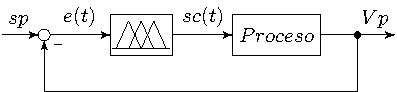
\includegraphics[width=0.9\textwidth]{pFuzzyTomo.pdf}
                    \caption[Esquema de control: P difuso]{\textbf{Esquema de control: P difuso}. Fuente: Elaboración propia.} 
                    \label{fig:pFuzzyTomo}
                \end{figure}

            \paragraph{Controlador PD difuso}
                
                Un controlador PD difuso puede ser realizado al tomar la señal de error y la derivada del error como entradas del controlador y se toma como salida la señal de control. El esquema de control se puede observar en la \cref{fig:pdFuzzyTomo}.

                \begin{figure}[htb]
                    \centering
                    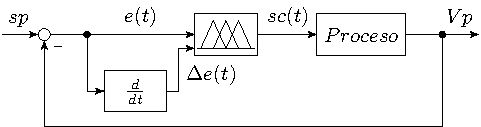
\includegraphics[width=0.9\textwidth]{pdFuzzyTomo.pdf}
                    \caption[Esquema de control: PD difuso]{\textbf{Esquema de control: PD difuso}. Fuente: Elaboración propia.} 
                    \label{fig:pdFuzzyTomo}
                \end{figure}
            
            \paragraph{Controlador PI difuso}
                
                Un controlador PI difuso se puede obtener al agregar un integrador a la salida de un PD difuso, de este modo $sc(t) = e(t) + \Delta e(t)$ se transforma en $sc(t) = \int_0^t e(\tau)d\tau + e(t)$ la cual sera tomada como la señal de control. El esquema de control se puede observar en la \cref{fig:piFuzzyTomo}.

                \begin{figure}[htb]
                    \centering
                    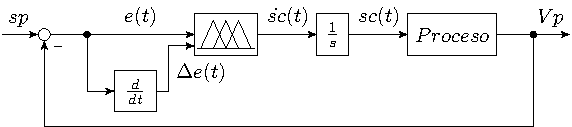
\includegraphics[width=0.9\textwidth]{piFuzzyTomo.pdf}
                    \caption[Esquema de control: PI difuso]{\textbf{Esquema de control: PI difuso}. Fuente: Elaboración propia.} 
                    \label{fig:piFuzzyTomo}
                \end{figure}

                \pagebreak

            \paragraph{Controlador PID difuso}
                
                Un controlador PD difuso puede ser realizado al tomar la señal de error, la derivada del error y la segunda derivada del error como entradas del controlador, la señal de salida es luego integrada de modo que $sc(t) = e(t) + \Delta e(t) + \Delta^2 e(t)$ se transforma en $sc(t) = \int_0^t e(\tau)d\tau + e(t) + \Delta e(t)$ la cual sera tomada como la señal de control. El esquema de control para un PID difuso completo se puede observar en la \cref{fig:pidFuzzyTomo}.

                \begin{figure}[htb]
                    \centering
                    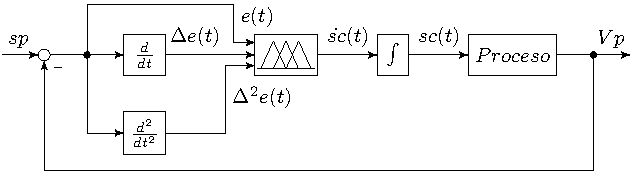
\includegraphics[width=0.9\textwidth]{pidFuzzyTomo.pdf}
                    \caption[Esquema de control: PID difuso]{\textbf{Esquema de control: PID difuso}. Fuente: Elaboración propia.} 
                    \label{fig:pidFuzzyTomo}
                \end{figure}

                Existen otras formas de obtener un PID difuso, una de estas formas es realizando la suma de las salidas de un PD difuso y PI difuso, por otro lado, tambien se puede realizar haciendo uso de componentes no difusos, i.e., sumar la salida de un PD difuso con la integral del error o sumar la salida de un PI difuso con la derivada del error.

            \paragraph{Controlador difuso como programador de ganancias}
                
                El esquema de control difuso con programdor de ganancias consiste en dos controladores, uno difuso y un PID clásico, el controlador difuso se encargará de generar las ganancias del PID de forma dinámica en función de las entradas que reciba, a su vez, el PID será quien gobierne al proceso, por lo cual permite adaptar el controlador PID a los cambios de carga y a los cambios del setpoint. El esquema de control se puede observar en la \cref{fig:GainschedulerTomo}.

                \begin{figure}[htb]
                    \centering
                    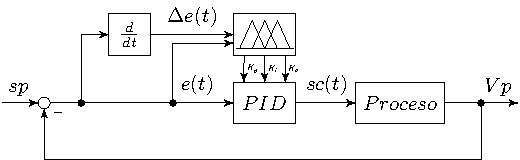
\includegraphics[width=0.8\textwidth]{GainschedulerTomo.pdf}
                    \caption[Esquema de control: Programador de ganancias]{\textbf{Esquema de control: Programador de ganancias}. Fuente: Elaboración propia.} 
                    \label{fig:GainschedulerTomo}
                \end{figure}
            
            \paragraph{Controlador combinado}
                
                Consiste en sumar las salidas de un controlador PID clasico y un controlador difuso, de este modo el controlador PID sera quien gobierne al proceso la mayoria del tiempo, para el caso de un controlador P difuso al generarce un cambio en el setpoint o la carga el controlador difuso procesedera a emitir una salida proporcional y adaptada al cambio. El esquema de control se puede observar en la \cref{fig:pidplusFuzzyTomo}.
            
                \begin{figure}[htb]
                    \centering
                    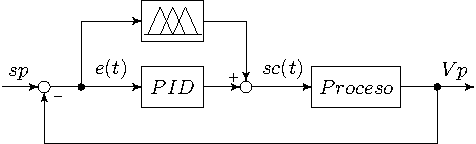
\includegraphics[width=0.8\textwidth]{pidplusFuzzyTomo.pdf}
                    \caption[Esquema de control: PID clasico mas difuso]{\textbf{Esquema de control: PID clasico mas difuso}. Fuente: Elaboración propia.} 
                    \label{fig:pidplusFuzzyTomo}
                \end{figure}

    \subsection{Python}
        
        Python es un lenguaje de programación interpretado y multiparadigma ya que soporta programación orientada a objetos, imperativa y en menor medida funcional. \textcite{guido2017tutorial} afirma que Python es un lenguaje de programación potente que puede aprenderse fácilmente. Cuenta con estructuras de datos eficientes y de alto
        nivel y un enfoque simple pero efectivo a la programación orientada a objetos. La elegante sintaxis de Python y su escritura
        dinámica, junto con su naturaleza interpretada, hacen de éste un lenguaje ideal para scripting y desarrollo rápido de
        aplicaciones en diversas áreas y sobre la mayoría de las plataformas.
        
        Adicionalmente, Python posee bibliotecas externas para realizar cálculos numéricos complejos, también existen bibliotecas para el análisis de sistemas de control y para el diseño de controladores difusos, por otro lado, existen bibliotecas para salidas gráficas con calidad de publicación, gráficas en tiempo real y en 3D.
        
        \subsubsection{Biblioteca NumPy}

            NumPy es una biblioteca para realizar cálculos computacionales científicos y matemáticos, algunas de sus funciones son: cálculo de vectores n-dimensionales, transformada de Fourier, álgebra lineal, entre otras \Parencite{numpy}

        \subsubsection{Biblioteca SciPy}	

            El paquete SciPy es un conjunto de bibliotecas matemáticas, científicas y de ingeniería compuestas por: NumPy, SciPy (biblioteca), SymPy, Matplotlib, IPython y Pandas, la biblioteca SciPy es uno de los núcleos del paquete SciPy. Provee varias rutinas eficientes de uso amigable para el usuario de tipo numérica para realizar integración, interpolación, optimización, álgebra lineal, estadísticas, entre otras \Parencite{scipy}, toda la documentación puede ser conseguida en la página oficial de SciPy.
            
        \subsubsection{Biblioteca Matplotlib}

            Matplotlib es una biblioteca para la graficación 2D que produce figuras con calidad de publicación en varios formatos y a través de múltiples ambientes interactivos. Matplotlib puede ser usado en scripting, consolas de comando, IPython, jupyter notebooks y en aplicaciones web \Parencite{Hunter:2007}. La sintaxis para usar Matplotlib es muy similar al sistema de plots de MATLAB, del mismo modo, configurar parámetros de estilos, fuentes, anchos de línea, entre otros, se realiza de manera similar.

        \subsubsection{Biblioteca de control}

            La biblioteca control de python es un conjunto de clases y funciones que implementan las operaciones más comunes en sistemas de control, además, posee un módulo de compatibilidad para usuarios de MATLAB que emula las funciones y sintaxis de este lenguaje \Parencite{pythoncontrol}. Para crear el modelo de un sistema podemos usar ecuaciones de espacio de estado o funciones de transferencia.

        \subsubsection{Biblioteca Scikit-Fuzzy}
            
            Scikit-Fuzzy es una colección de algoritmos de lógica difusa con la intención de pertenecer al paquete de herramientas científicas SciPy, esta biblioteca permite diseñar y simular controladores difusos con estructura tipo Mamdani \Parencite{warner2016fuzzy}, no posee un modo para realizar lazos de control o compatibilidad con la biblioteca de control de forma directa, de modo que se tendrían que codificar aparte las rutinas que conformen un lazo cerrado de control.

        \subsubsection{Biblioteca PySide2}

            PySide2 es una biblioteca que hace de union entre Qt y Python para la creacion de interfacez de usuario. PySide2 es soportado por linux, Mac OS x, windows, entre otros.
            
        \subsubsection{Biblioteca PyQtGraph}
                
            PyQtGraph es una biblioteca de graficacion especializada en graficas dinamicas y en tiempo real, utiliza de fondo un nucleo Qt, por tanto, requiere el uso de PyQt4, PyQt5, PySide o PySide2. 

\chapter{Marco metodológico}
	En este capítulo se abarcará la metodología a emplear en el desarrollo de esta investigación, se definirá el tipo, diseño y modalidad de la investigación, así como las fases de la misma.

\section{Tipo de investigación}
	
	Tomando en cuenta los objetivos de la investigación y las bases teóricas que la componen se considera que esta investigación es de tipo proyectiva, esto es debido a que se pretende realizar una propuesta concreta para solventar una problemática, \textcite{jacquelin2010guia} afirma que:	
	
	\blockquote[p.$\,$133]{La investigación proyectiva tiene como objetivo diseñar o crear propuestas dirigidas a resolver determinadas situaciones. Los proyectos de arquitectura e ingeniería, el diseño de maquinarias, la creación de programas de intervención social, el diseño de programas de estudio, los inventos, la elaboración de programas informáticos, entre otros, siempre que estén sustentados en un proceso de investigación, son ejemplos de investigación proyectiva.}

\section{Diseño de la investigación}

	El diseño de la investigación es no experimental y de tipo transeccional descriptivo, esto es debido a que se describirán los métodos de análisis y diseño de sistemas de control clásicos y difusos, \textcite{sampieri1998metodologia} definen la investigación no experimental como: \blockquote[p.150]{la investigación que se realiza sin manipular deliberadamente variables. Es decir,
	se trata de estudios donde no hacemos variar en forma intencional las variables independientes para
	ver su efecto sobre otras variables. Lo que hacemos en la investigación no experimental
	es observar fenómenos tal como se dan en su contexto natural, para posteriormente
	analizarlos.}

\section{Modalidad}

	Esta investigación se encuentra enmarcada en la modalidad de un proyecto factible, debido a que tiene objetivos para atender una necesidad por medio de unas acciones claramente definidas, \textcite{renie2002factible} afirma que:
	
	\blockquote[pp.$\,$6-7]{un proyecto factible consiste en un conjunto de actividades vinculadas entre sí, cuya ejecución permitirá el logro de objetivos previamente definidos en atención a las necesidades que pueda tener una institución o un grupo social en un momento determinado. Es decir, la finalidad del proyecto factible radica en el diseño de una propuesta de acción dirigida a resolver un problema o necesidad previamente detectada en el medio.}

\section{Fases de la investigación}
	
	\paragraph{Fase 1: Estudio de los sistemas de control clásicos y difusos}
		
		En esta fase se procederá a realizar los estudios necesarios en el área de los sistemas de control, esto con la idea de abarcarlos en profundidad y tener un entendimiento claro de su funcionamiento y de la matemática implicada, además, se realizará de forma similar un estudio de controladores difusos con estructura Mamdani y de los esquemas de control difuso.
		
	\paragraph{Fase 2: Codificación de rutinas}
		
		Para esta fase con los conocimientos adquiridos de la fase 1, se determinarán que rutinas pueden ser ejecutadas solo con las bibliotecas de python y cuales se deberán codificar de cero, además, se codificaran todas las rutinas necesarias para el funcionamiento del laboratorio virtual, para esto, se hará uso de las bibliotecas externas de cálculo numérico, control, diseño de controladores difusos y salidas gráficas junto con las que se consideren necesarias.
		
	\paragraph{Fase 3: Interfaz gráfica y enlace con rutinas}
		
		En esta fase se realizará la interfaz gráfica para el usuario final, esta interfaz gráfica deberá conectarse y adaptarse a las rutinas previamente codificadas en la fase 2 para su funcionamiento adecuado, en orden de tener diseño acorde se tomarán en cuenta los antecedentes presentados en esta propuesta.
		
	\paragraph{Fase 4: Comparación de resultados}
		
		En esta última fase y con el laboratorio de sistemas de control, ya en funcionamiento, se procederá a analizar los resultados obtenidos y a compararlos con otras herramientas, la evaluación se realizará en función del resultado esperado, facilidad de implementación, velocidad de ejecución, las ventajas y desventajas de cada una de las herramientas.

\section{Aspectos administrativos}

		\subsubsection{Factibilidad de la propuesta}

		Esta investigación es claramente factible al estar enfocada en la utilización de software libre para la creación del laboratorio virtual, así lo demuestran los antecedentes expuestos en esta propuesta, los cuales han hecho uso de software para le creación de aplicaciones con usos en el área de los sistemas de control, otros han utilizado específicamente Python para el desarrollo de controladores difusos, además, al tratarse de software libre no existe la necesidad de financiación externa, facilitando así su desarrollo. Para realizar esta investigación solo hará falta el uso de una computadora con acceso a internet con el fin de obtener el software necesario y realizar las investigaciones pertinentes en cada tema, así mismo se espera hacer uso de la biblioteca de la universidad, nuevamente, para realizar las investigaciones pertinentes.
		
	\subsubsection{Cronograma de ejecución}

		Las actividades a realizar fueron determinadas en función de las fases, los requerimientos y objetivos de esta investigación, en la \cref{tab:Cronograma} se puede observar el cronograma de ejecución, en donde se denotan las fases y actividades de la misma junto con el número de semanas que se estima emplear en cada una de las actividades. La estimación de semanas para cada una de las actividades se tomó considerando la complejidad del tema, a su vez, la complejidad fue evaluada tomando en cuenta los antecedentes expuestos en esta propuesta y teniendo en consideración las experiencias similares previas en cada uno de los temas a abarcar.

		Adicionalmente, se realizó un diagrama de Gantt para tener una mejor representación de la dependencia entre actividades, así como de los tiempos a utilizar en cada actividad durante el desarrollo de la investigación. El diagrama se puede observar en la \cref{fig:gantt}, a continuación se listan las actividades a realizar:

		\vspace{10pt}

		\begin{enumerate}[label=\bfseries Actividad \arabic*:, wide=0pt, leftmargin=*]
			\item Estudio de los métodos de análisis de sistemas de control. 
			\item Estudio de controladores PID.
			\item Estudio de controladores difusos tipo Mamdani.
			\item Codificar las rutinas de análisis de sistemas de control.
			\item Codificar las rutinas para la entonación de controladores PID.
			\item Codificar rutinas para la creación de controladores difusos.
			\item Codificar rutinas para la simulación de sistemas de control.
			\item Crear la interfaz gráfica para el laboratorio virtual.
			\item Acoplar las rutinas con la interfaz gráfica.
			\item Análisis de resultados obtenidos.
			\item Comparación con otras herramientas.
		\end{enumerate}

\afterpage{
\begin{landscape}
\begin{table}
    \caption{Cronograma de ejecución}
    \label{tab:Cronograma}
    \small
    \begin{tabular}{@{\extracolsep{\fill}}llc}
    \toprule
    \multicolumn{1}{c}{Fases} & \multicolumn{1}{c}{Actividades} & \multicolumn{1}{l}{Semanas} \\ \midrule
    \multirow{3}{*}{Fase 1: Estudio de los sistemas de control clásicos y difusos} & Estudio de los métodos de análisis de sistemas de control & 1 \\
     & Estudio de controladores PID & 1 \\
     & Estudio de controladores difusos tipo Mamdani & 1 \\
     &  & \multicolumn{1}{l}{} \\
    \multirow{4}{*}{Fase 2: Codificación de rutinas} & Codificar las rutinas de análisis de sistemas de control & 2 \\
     & Codificar las rutinas para la entonación de controladores PID & 1 \\
     & Codificar rutinas para la creación de controladores difusos & 2 \\
     & Codificar rutinas para la simulación de sistemas de control & 2 \\
     &  & \multicolumn{1}{l}{} \\
    \multirow{2}{*}{Fase 3: Interfaz gráfica y enlace con rutinas} & Crear la interfaz gráfica para el laboratorio virtual & 1 \\
     & Acoplar las rutinas con la interfaz gráfica & 4 \\
     &  & \multicolumn{1}{l}{} \\
    \multirow{2}{*}{Fase 4: Comparación de resultados} & Análisis de resultados obtenidos & 1 \\
     & Comparación con otras herramientas & 1 \\ \midrule
     & \multicolumn{1}{r}{Total semanas:} & 17 \\ \bottomrule
    \end{tabular}%
\end{table}
\end{landscape}
}

\newganttlinktypealias{straight}{f-s}
\setganttlinklabel{straight}{}

\afterpage{
\begin{landscape}
	\begin{figure}
	\begin{ganttchart}[
				hgrid,
				vgrid={*{6}{draw=none},dotted},
				%today=15,%
				%today offset=.5,%
				%today label=Heute,%
				%progress=today,%
				x unit=4.2pt,
				y unit chart=0.6cm,
				newline shortcut=true,
				bar/.append style={gray!33},
				canvas/.append style={fill=none},
				group/.style={fill=gray},
				link bulge = 1.3,
        		link/.style={-to, rounded corners = 3pt, thick},
				]{1}{119}
	
	\gantttitle{2019}{119} \\
	\gantttitle{Julio}{21}
	\gantttitle{Agosto}{31}
	\gantttitle{Septiembre}{30}
	\gantttitle{Octubre}{31}
	\gantttitle{Nov}{6}\\
	\gantttitle{W1}{7}
	\gantttitle{W2}{7}
	\gantttitle{W3}{7}
	\gantttitle{W4}{7}
	\gantttitle{W5}{7}
	\gantttitle{W6}{7}
	\gantttitle{W7}{7} 
	\gantttitle{W8}{7}
	\gantttitle{W9}{7}
	\gantttitle{W10}{7}
	\gantttitle{W11}{7}
	\gantttitle{W12}{7}
	\gantttitle{W13}{7}
	\gantttitle{W14}{7}
	\gantttitle{W15}{7}
	\gantttitle{W16}{7}
	\gantttitle{W17}{7}\\

	\ganttgroup{Duracion Total}{1}{119} \\
	
	\ganttgroup{Fase 1}{1}{21} \\
	\ganttbar{Actividad 1}{1}{7} \\
	\ganttbar{Actividad 2}{8}{14} \\
	\ganttbar{Actividad 3}{15}{21} \\
	
	\ganttgroup{Fase 2}{22}{70}\\
	\ganttbar{Actividad 4}{22}{35} \\
	\ganttbar{Actividad 5}{36}{42} \\
	\ganttbar{Actividad 6}{43}{56} \\
	\ganttbar{Actividad 7}{57}{70} \\
	
	\ganttgroup{Fase 3}{71}{105} \\
	\ganttbar{Actividad 8}{71}{77} \\
	\ganttlinkedbar[link bulge=3, link type=straight]{Actividad 9}{78}{105} \\

	\ganttgroup{Fase 4}{106}{119} \\
	\ganttbar{Actividad 10}{106}{112} \\
	\ganttlinkedbar[link bulge=3, link type=straight]{Actividad 11}{113}{119} \\
	
	\begin{scope}[on background layer]
	\ganttlink[link bulge=3]{elem2}{elem6}
	\ganttlink[link bulge=3]{elem3}{elem7}
	\ganttlink[link bulge=3]{elem4}{elem8}
	
	\ganttlink[link bulge=3]{elem2}{elem9}
	\ganttlink[link bulge=3]{elem3}{elem9}
	\ganttlink[link bulge=3]{elem4}{elem9}

	\ganttlink[link bulge=3]{elem6}{elem12}
	\ganttlink[link bulge=3]{elem7}{elem12}
	\ganttlink[link bulge=3]{elem8}{elem12}
	\ganttlink[link bulge=3]{elem9}{elem12}
	\ganttlink[link bulge=3, link type=straight]{elem12}{elem14}
	\end{scope}
	\end{ganttchart}
	\caption[Diagrama de Gantt]{\textbf{Diagrama de Gantt}. Donde \enquote{W} denota las semanas, con un total de 17 semanas y tomando la fecha de inicio como el 10-07-2019, la fecha de finalización seria el 06-11-2019. Fuente: Elaboración propia}
	\label{fig:gantt}
	\end{figure}
	\end{landscape}
}



% ------------------------------ fin -----------------------------------

%\backmatter
\FrontBackStyle
\CenterformatBack
\addtocontents{toc}{\vspace{0.6\normalbaselineskip}}

%\newpage
%\CenterformatFront
\singlespacing
\printbibliography[title={REFERENCIAS},heading=bibintoc]	% referencias , heading=bibnumbered para numeración

%\spacing{1.5}
%\chapter{ANEXOS}

\end{document}